%%%%%%%%%%%%%%%%%%%%%%%%%%%%%%%%%%%%%%%%%
% Masters/Doctoral Thesis 
% LaTeX Template
% Version 2.5 (27/8/17)
%
% This template was downloaded from:
% http://www.LaTeXTemplates.com
%
% Version 2.x major modifications by:
% Vel (vel@latextemplates.com)
%
% This template is based on a template by:
% Steve Gunn (http://users.ecs.soton.ac.uk/srg/softwaretools/document/templates/)
% Sunil Patel (http://www.sunilpatel.co.uk/thesis-template/)
%  
% Template license:
% CC BY-NC-SA 3.0 (http://creativecommons.org/licenses/by-nc-sa/3.0/)
%
%%%%%%%%%%%%%%%%%%%%%%%%%%%%%%%%%%%%%%%%%

%----------------------------------------------------------------------------------------
%	PACKAGES AND OTHER DOCUMENT CONFIGURATIONS
%----------------------------------------------------------------------------------------

\documentclass[
12pt, % The default document font size, options: 10pt, 11pt, 12pt
oneside, % Two side (alternating margins) for binding by default, uncomment to switch to one side
english, % ngerman for German
onehalfspacing, % Single line spacing, alternatives: onehalfspacing or doublespacing
%draft, % Uncomment to enable draft mode (no pictures, no links, overfull hboxes indicated)
nolistspacing, % If the document is onehalfspacing or doublespacing, uncomment this to set spacing in lists to single
%liststotoc, % Uncomment to add the list of figures/tables/etc to the table of contents
%toctotoc, % Uncomment to add the main table of contents to the table of contents
%parskip, % Uncomment to add space between paragraphs
%nohyperref, % Uncomment to not load the hyperref package
headsepline, % Uncomment to get a line under the header
%chapterinoneline, % Uncomment to place the chapter title next to the number on one line
%consistentlayout, % Uncomment to change the layout of the declaration, abstract and acknowledgements pages to match the default layout
addchap,
]{MastersDoctoralThesis} % The class file specifying the document structure

\usepackage[utf8]{inputenc} % Required for inputting international characters
\usepackage[T1]{fontenc} % Output font encoding for international characters
\usepackage[utf8]{vietnam}
\usepackage{amsthm, amsmath}
\usepackage{commath}
\usepackage{array}
\usepackage{booktabs}
\newcolumntype{C}[1]{>{\centering\let\newline\\\arraybackslash\hspace{0pt}}m{#1}}
\usepackage{caption}
\usepackage{subcaption}
\usepackage{tikz,pgfplots}
\usetikzlibrary{arrows, shapes, calc, fit, positioning, backgrounds}
\usepackage[vietnam]{minitoc}
\usepackage{enumitem}
\usepackage[ruled]{algorithm2e} %dotocloa
\renewcommand{\algorithmcfname}{Thuật toán}
\renewcommand{\listalgorithmcfname}{Danh sách thuật toán}
\SetKwInput{KwInput}{Khởi tạo}

\usepackage{mathpazo} % Use the Palatino font by default
\usepackage{times}

\usepackage[backend=bibtex,style=ieee,natbib=true]{biblatex} % Use the bibtex backend with the authoryear citation style (which resembles APA)

\addbibresource{Includes/references} 
% Define some commands to keep the formatting separated from the content 
\newcommand{\keyword}[1]{\textbf{#1}}
\newcommand{\tabhead}[1]{\textbf{#1}}
\newcommand{\code}[1]{\texttt{#1}}
\newcommand{\file}[1]{\texttt{\bfseries#1}}
\newcommand{\option}[1]{\texttt{\itshape#1}}

\newcommand{\ra}{\rightarrow}
\newcommand{\Ra}{\Rightarrow}
\newcommand{\lra}{\longrightarrow}
\newcommand{\Lra}{\Longrightarrow}
\newcommand{\la}{\leftarrow}
\newcommand{\La}{\Leftarrow}
\newcommand{\lla}{\longleftarrow}
\newcommand{\Lla}{\Longleftarrow}
\newcommand{\Llra}{\Longleftrightarrow}
\newcommand{\map}{\longmapsto}

\newcommand{\pa}{\partial}
\newcommand{\al}{\alpha}
\newcommand{\bt}{\beta}
\newcommand{\de}{\delta}
\newcommand{\De}{\Delta}
\newcommand{\tta}{\theta}
\newcommand{\e}{\varepsilon}
\newcommand{\vp}{\varphi}
\newcommand{\na}{\nabla}
\newcommand{\sm}{\sigma}
\newcommand{\Sm}{\Sigma}
\newcommand{\gm}{\gamma}
\newcommand{\Gm}{\Gamma}
\newcommand{\Om}{\Omega}
\newcommand{\R}{\mathbb R}
\newcommand{\Q}{\mathbb Q}
\newcommand{\N}{\mathbb N}
\newcommand{\Z}{\mathbb Z}
\newcommand{\Pp}{\mathbb P}
\newcommand{\Oo}{\mathcal O}
\newcommand{\K}{\mathcal K}
\newcommand{\GG}{\mathcal G}
\newcommand{\DD}{\mathcal D}
\newcommand{\XX}{\mathcal X}
\newcommand{\MM}{\mathcal M}
\newcommand{\TT}{\mathcal T}
\newcommand{\VV}{\mathcal V}
\newcommand{\WW}{\mathcal W}
\newcommand{\UU}{\mathcal U}
\newcommand{\PP}{\mathcal P}
\newcommand{\LL}{\mathcal L}
\newcommand{\BB}{\mathcal B}
\newcommand{\CC}{\mathcal C}
\newcommand{\KK}{\mathcal K}
\newcommand{\HH}{\mathcal H}
\newcommand{\EE}{\mathcal E}
\newcommand{\QQ}{\mathcal Q}
\newcommand{\cbe}{\scriptsize}
\newcommand{\On}{\widetilde{\mathcal{O}}}
\newcommand{\Mn}{\widetilde{M}}
\newcommand{\sumh}{\overline{\sum}}
\newcommand{\cho}[2]{\ensuremath{#1\choose#2}}
\newcommand{\ve}[1]{{\bf #1}}
\newcommand{\wt}[1]{\widetilde #1}
%\newcommand{\norm}[1]{\left\lVert#1\right\rVert}

\newtheorem{thm}{Định lý}[chapter]
\newtheorem{hypo}{Giả thuyết}
\newtheorem{nota}{Ký hiệu}[chapter]
\newtheorem{lem}{Bổ đề}[chapter]
\newtheorem{prop}{Mệnh đề}[chapter]
\newtheorem{coro}{Hệ quả}[thm]
\newtheorem{defi}{Định nghĩa}[chapter]
\newtheorem{exam}{Ví dụ}[chapter]
\newtheorem{rem}{Nhận xét}[chapter]
\newtheorem{pro}{Tính chất}[defi]

\DeclareMathOperator{\essup}{essup}
\DeclareMathOperator{\Div}{div}
\DeclareMathOperator{\Rot}{rot}
\DeclareMathOperator{\nv}{n}
\DeclareMathOperator{\Vol}{Vol}
\DeclareMathOperator{\Per}{Per}


\usepackage[autostyle=true]{csquotes} % Required to generate language-dependent quotes in the bibliography

\usepackage{tocloft}

% Leaders for chapter entries
\renewcommand\cftchapdotsep{\cftdotsep}
\renewcommand\cftfigdotsep{\cftdotsep}
\renewcommand\cfttabdotsep{\cftdotsep}


% Add space to account for new chapter numbering schema
\renewcommand\cftchapnumwidth{6em}
\renewcommand\cftfignumwidth{5em}
\renewcommand\cfttabnumwidth{5em}


% Redefine representation for chapter (and section) counters
\renewcommand\cftchappresnum{Chương }
\renewcommand\cftfigpresnum{\em Hình }
\renewcommand\cfttabpresnum{\em Bảng }

%----------------------------------------------------------------------------------------
%	MARGIN SETTINGS
%----------------------------------------------------------------------------------------

\geometry{
	paper=a4paper, % Change to letterpaper for US letter
	%inner=2.5cm, % Inner margin
	%outer=3.8cm, % Outer margin
	bindingoffset=.5cm, % Binding offset
	%top=1.5cm, % Top margin
	%bottom=1.5cm, % Bottom margin
	%showframe, % Uncomment to show how the type block is set on the page
	top=3.5cm, bottom=3cm,inner=3.5cm, outer=2cm
}
\renewcommand{\baselinestretch}{1.5}

%----------------------------------------------------------------------------------------
%	THESIS INFORMATION
%----------------------------------------------------------------------------------------

\thesistitle{Mô phỏng biến dạng đàn hồi bằng phương pháp phần tử hữu hạn và ứng dụng trong công nghiệp vật liệu} % Your thesis title, this is used in the title and abstract, print it elsewhere with \ttitle
\supervisor{TS. Tạ Thị Thanh \textsc{Mai}} % Your supervisor's name, this is used in the title page, print it elsewhere with \supname
\examiner{} % Your examiner's name, this is not currently used anywhere in the template, print it elsewhere with \examname
\degree{Thạc sĩ Khoa học Toán ứng dụng} % Your degree name, this is used in the title page and abstract, print it elsewhere with \degreename
\author{Nguyễn Lê \textsc{Hoàng}} % Your name, this is used in the title page and abstract, print it elsewhere with \authorname
\addresses{} % Your address, this is not currently used anywhere in the template, print it elsewhere with \addressname

\subject{Toán ứng dụng} % Your subject area, this is not currently used anywhere in the template, print it elsewhere with \subjectname
\keywords{cơ học vật liệu, phương trình đàn hồi, phương pháp phần tử hữu hạn, \code{Freefem++}} % Keywords for your thesis, this is not currently used anywhere in the template, print it elsewhere with \keywordnames
\university{\href{http://www.hust.edu.vn}{ĐẠI HỌC BÁCH KHOA HÀ NỘI}} % Your university's name and URL, this is used in the title page and abstract, print it elsewhere with \univname
\department{\href{http://sami.hust.edu.vn/don-vi/bo-mon-toan-ung-dung/gioi-thieu/}{Bộ môn Toán ứng dụng}} % Your department's name and URL, this is used in the title page and abstract, print it elsewhere with \deptname
\group{\href{http://www.sami.hust.edu.vn}{}}
%\group{\href{http://researchgroup.university.com}{Research Group Name}} % Your research group's name and URL, this is used in the title page, print it elsewhere with \groupname
\faculty{\href{http://www.sami.hust.edu.vn}{Viện Toán ứng dụng và Tin học}} % Your faculty's name and URL, this is used in the title page and abstract, print it elsewhere with \facname

\AtBeginDocument{
\hypersetup{pdftitle=\ttitle} % Set the PDF's title to your title
\hypersetup{pdfauthor=\authorname} % Set the PDF's author to your name
\hypersetup{pdfkeywords=\keywordnames} % Set the PDF's keywords to your keywords
}

\begin{document}
%\setcounter{chapter}{-1}
\dominitoc
\frontmatter % Use roman page numbering style (i, ii, iii, iv...) for the pre-content pages

\pagestyle{plain} % Default to the plain heading style until the thesis style is called for the body content

%----------------------------------------------------------------------------------------
%	TITLE PAGE
%----------------------------------------------------------------------------------------

\begin{titlepage}
\begin{center}

\vspace*{.04\textheight}
{\scshape\LARGE \univname\par}\vspace{1.35cm} % University name
\textsc{\Large Luận Văn Thạc Sĩ}\\[0.2cm] % Thesis type

\HRule \\[-0.1cm] % Horizontal line
{\huge \bfseries \ttitle\par}\vspace{0.1cm} % Thesis title
\HRule \\[1cm] % Horizontal line
 
\begin{minipage}[t]{0.4\textwidth}
\begin{flushleft} \large
\emph{Học viên:}\\
\href{hoangnl.w@gmail.com}{\authorname} % Author name - remove the \href bracket to remove the link
\end{flushleft}
\end{minipage}
\begin{minipage}[t]{0.4\textwidth}
\begin{flushright} \large
\emph{Giảng viên hướng dẫn:} \\
\href{mai.tathithanh@hust.edu.vn}{\supname} % Supervisor name - remove the \href bracket to remove the link  
\end{flushright}
\end{minipage}\\[1.5cm] 
\vfill

\large \textit{Luận văn được thực hiện trong chương trình \\\degreename}\\ % University requirement text
\textit{tại}\\
%\groupname\\
\facname \\[1cm] % Research group name and department name
 
\vfill

{\large \today}\\[3.5cm] % Date
 
\vfill
\end{center}
\end{titlepage}

%----------------------------------------------------------------------------------------
%	DECLARATION PAGE
%----------------------------------------------------------------------------------------

\begin{declaration}
%\addstarredchapter{\authorshipname}
%\addstarredchapter{Lời cam đoan}
%\addchaptertocentry{\authorshipname} % Add the declaration to the table of contents
\noindent Tôi, \textbf{Nguyễn Lê Hoàng}, cam đoan rằng luận văn thạc sĩ với tiêu đề \enquote{\em{\ttitle}} là công trình nghiên cứu khoa học của riêng tôi. Tôi xin xác nhận rằng:

\begin{itemize} 
\item Luận văn này được thực hiện chủ yếu trong chương trình Thạc sĩ Khoa học Toán ứng dụng tại Viện Toán ứng dụng và Tin học, Đại học Bách Khoa Hà Nội.
\item Bất kỳ nội dung nào của luận văn này được sử dụng trong bất kỳ tài liệu nào khác đã được nêu rõ ràng.
\item Tất cả các tài liệu được sử dụng để tham khảo đã được trích dẫn đầy đủ. Ngoài các trích dẫn đó, luận văn này hoàn toàn là kết quả của tôi cùng nhóm nghiên cứu.
\item Mọi sự giúp đỡ trong quá trình thực hiện luận văn đều đã được ghi nhận và cảm ơn.\\\\\\
\end{itemize}
 
\noindent Chữ ký:\\
\rule[0.5em]{20em}{0.5pt} % This prints a line for the signature
\\
\noindent Ngày: \\
\rule[0.5em]{20em}{0.5pt} % This prints a line to write the date
%\\[8cm]
\end{declaration}\\

\cleardoublepage

%----------------------------------------------------------------------------------------
%	ABSTRACT PAGE
%----------------------------------------------------------------------------------------

\begin{abstract}
%\addcontentsline{toc}{chapter}{Tóm tắt nội dung} 
\addstarredchapter{Tóm tắt nội dung}
%\addchaptertocentry{\abstractname} % Add the abstract to the table of contents
Trong luận văn này, tác giả trình bày một thuật toán giải số cho bài toán biến dạng đàn hồi. Phần đầu tiên trình bày về mô phỏng số cho phương trình đàn hồi dựa trên phương pháp phần tử hữu hạn. Phần hai là một số ví dụ mô phỏng số cho phương trình đàn hồi và một vài ứng dụng trong công nghiệp vật liệu. Mã nguồn chương trình được phát triển trên phần mềm \code{Freefem++}, dựa trên phương pháp phần tử hữu hạn.\\

\noindent \textbf{Từ khóa:} \keywordnames
\end{abstract}


%----------------------------------------------------------------------------------------
%	ACKNOWLEDGEMENTS
%----------------------------------------------------------------------------------------

\begin{acknowledgements}
%\addstarredchapter{Lời cảm ơn}

Lời đầu tiên, tác giả xin bày tỏ lòng biết ơn chân thành và sâu sắc nhất tới TS. \textbf{Tạ Thị Thanh Mai}, người đã tận tình hướng dẫn, giúp đỡ và động viên tác giả trong suốt quá trình thực hiện luận văn này.\\[-0.5cm]

Tác giả xin trân trọng cảm ơn Viện Toán ứng dụng và Tin học, Viện Đào tạo Sau đại học, Đại học Bách Khoa Hà Nội đã tạo mọi điều kiện thuận lợi cho tác giả trong quá trình học tập và nghiên cứu. Xin cảm ơn các thầy cô, các bạn sinh viên, học viên cao học của Viện Toán ứng dụng và Tin học đã giúp đỡ, trao đổi cùng tác giả những kiến thức và kinh nghiệm quý báu để giúp cho luận văn này được hoàn thiện hơn. Tác giả cũng xin gửi lời cảm ơn chân thành tới bạn \textbf{H} đã cộng tác và giúp đỡ tác giả trong quá trình nghiên cứu và thực hiện đề tài.\\[-0.5cm]

Cuối cùng, tác giả xin kính tặng những người thân yêu nhất của mình niềm hạnh phúc và vinh dự to lớn này!
\end{acknowledgements}
\newpage
%----------------------------------------------------------------------------------------
%	LIST OF CONTENTS/FIGURES/TABLES PAGES
%----------------------------------------------------------------------------------------
\renewcommand{\baselinestretch}{1.25}
\tableofcontents % Prints the main table of contents
\renewcommand{\baselinestretch}{1.5}

\newpage
\listoffigures % Prints the list of figures
%\addstarredchapter{Danh sách hình vẽ}

\newpage
\listoftables % Prints the list of tables
%\addstarredchapter{Danh sách bảng}

\newpage
\listofalgorithms % Prints the list of algorithms
%\addstarredchapter{Danh sách thuật toán}

%----------------------------------------------------------------------------------------
%	SYMBOLS
%----------------------------------------------------------------------------------------
%\begin{symbols}{ll} % Include a list of Symbols (a three column table)
%Symbol & Name \\
$\N$	& Tập hợp các số tự nhiên. \\
$\R$	& Tập hợp các số thực. \\
$\R^+$	& Tập hợp các số thực không âm.\\
$\R^d$	& Không gian Euclide $d$ chiều.\\
$\emptyset$	& Tập hợp rỗng.\\
$\dim V$	& Số chiều của không gian hữu hạn chiều $V$.\\
\addlinespace
$\Om$	& Miền bị chặn trong không gian $\R^d$.\\
$\pa\Om$ & Biên của miền $\Om$.\\
$\nv$ & Vector pháp tuyến đơn vị của biên. \\
$\tau$ & Vector tiếp tuyến đơn vị của biên. \\
$\Vol(\Om)$ & Thể tích của miền $\Om$ (tương ứng diện tích trong $\R^2$). \\
$\Per(\Om)$ & Chu vi của miền $\Om$. \\
\addlinespace
\addlinespace
$\na f$			& Ma trận gradient của hàm $f:\R^d \ra \R^d$.\\
$\Delta f$		& Toán tử Laplace của hàm $f$: $\Delta f = \displaystyle \dfrac{\pa^2 f_1}{\pa x_1^2} + \dfrac{\pa^2 f_2}{\pa x_2^2} +\cdots + \dfrac{\pa^2 f_d}{\pa x_d^2}$.\\
$\Div f$		& Toán tử vector: $\Div f = \displaystyle \dfrac{\pa f_1}{\pa x_1} + \dfrac{\pa f_2}{\pa x_2} +\cdots + \dfrac{\pa f_d}{\pa x_d}$.\\
$\Rot f$		& Toán tử vector. Trường hợp $d = 2: \Rot f = \displaystyle \dfrac{\pa f_2}{\pa x_1} - \dfrac{\pa f_1}{\pa x_2}$.\\
\addlinespace
$u\cdot \na$ & Toán tử hình thức: $(u\cdot \na)v = \na v.u$ .\\
$u\cdot v$		& Tích vô hướng của hai vector trong $\R^d$: $u\cdot v = \displaystyle \sum_{i=1}^d u_iv_i$.\\
$A:B$			& Tích vô hướng Frobenius của hai ma trận: $A: B = \displaystyle \sum_{i,j=1}^d A_{ij}B_{ij}$.\\
\addlinespace
$\underset{x \in E}{\essup}\, u(x)$ & Cận trên cốt yếu: $\underset{x \in E}{\essup}\, u(x) = \underset{\vert F\vert = 0}{\inf} ( \underset{x \in E\setminus F}{\sup}\, u(x) )$.\\
$\alpha$	& Vector đa chỉ số $\alpha = \left\lbrace\alpha_1,\ldots,\alpha_d \right\rbrace, \alpha_i \in \N$ với cấp $\vert \alpha\vert = \displaystyle\sum_{i=1}^d\alpha_i$.\\
$D^\alpha u$		& Đạo hàm theo đa chỉ số: $\displaystyle\alpha: D^\alpha u = \dfrac{\pa^{\left\vert\alpha\right\vert}u}{\pa x_1^{\alpha_1}\cdots\pa x_d^{\alpha_d}}$.\\
\addlinespace
$C^k(E)$			& Không gian các hàm thực có đạo hàm đến cấp $k$ liên tục trên $E$. \\
$L^p\left(E\right)$ &  Không gian hàm: $L^p\left(E\right) = \left\lbrace  u:E \ra \R \left\vert \displaystyle\int_E \vert u(x)\vert^p\,dx < \infty \right.\right\rbrace$. \\
$L^\infty\left(E\right)$ &  Không gian hàm: $L^\infty\left(E\right) = \left\lbrace  u:E \ra \R \vert\, \underset{x \in E}{\essup}\,\,  \vert u(x)\vert < \infty\right\rbrace$. \\
$W^{k, p}\left(E\right)$ & Không gian Sobolev: $\left\lbrace u:E\ra \R \left\vert \displaystyle D^\alpha u  \in L^p(E),\,\forall \left\vert\alpha\right\vert \leq k \right.\right\rbrace$.\\
$H^1\left(E\right)$ & Không gian Sobolev $H^1\left(E\right) := W^{1, 2}\left(E\right)$.  \\
$H^2\left(E\right)$ & Không gian Sobolev $H^2\left(E\right) := W^{2, 2}\left(E\right)$.  \\
$L^q\left(\TT; W^{k,p}(E)\right)$ & Không gian: $\left\lbrace u\in L^q\left(E \times \TT\right) \left\vert u(x, t) \in W^{k, p}\left(E\right),\, \forall t \in \TT\right.\right\rbrace$.\\
$W^{k, p}(\R^d, \R^d)$ & Không gian hàm: $\left\lbrace f:\R^d\ra \R^d \left\vert \forall i:  f_i(x) \in W^{k, p}(\R^d)\right.\right\rbrace$.\\
\addlinespace
$(\cdot, \cdot)$		& Tích vô hướng trong không gian $L^2(\Om)$: $(u, v) = \displaystyle \int_\Om uv \,\,dx$.\\
$\norm{\cdot}_0$ &  Chuẩn trong không gian $L^2(\Om):\norm{\cdot}_0 = \left(\displaystyle\int_\Om \vert\cdot\vert^2 \,dx\right)^{1/2}$.\\
$\norm{\cdot}_1$ & Chuẩn trong không gian $H^1(\Om) : \norm{\cdot}_1 = \left( \norm{\cdot}_0^2 + \norm{\na \cdot}_0^2 \right)^{1/2}$.\\
$\norm{\cdot}_2$ & Chuẩn trong không gian $H^2(\Om) : \norm{\cdot}_2 = \left( \displaystyle\sum_{0 \leq \vert\alpha\vert \leq 2} \norm{D^\alpha \cdot}_0^2 \right)^{1/2}$.\\
$\norm{\cdot}_\infty$ & Chuẩn trong không gian $L^\infty\left(E\right): \norm{\cdot}_\infty = \underset{x \in E}{\essup}\, \vert\cdot\vert$.\\
\addlinespace
\addlinespace
vđk.		& Viết tắt của cụm từ "với điều kiện". \\
\end{symbols}



%----------------------------------------------------------------------------------------
%	THESIS CONTENT - CHAPTERS
%----------------------------------------------------------------------------------------

\mainmatter 

\pagestyle{thesis} 
\chapter*{\centering Lời nói đầu}
\addstarredchapter{Lời nói đầu}
Bài toán biến dạng đàn hồi có ứng dụng rộng rãi trong cơ học vật liệu đặc biệt đối với các vấn đề liên quan đến độ bền, ứng suất và biến dạng. Độ bền của vật liệu là khả năng chịu đựng không bị nứt, gãy, phá hủy hay biến dạng dẻo dưới tác động của ngoại lực bên ngoài. Tùy theo các ngoại lực khác nhau mà đặc tính về độ bền của vật liệu cũng khác nhau: độ kéo, độ bền nén, độ bền cắt, độ bền uốn, độ bền mỏi, độ bền va đập, giới hạn chảy...\\
Phương pháp phần tử hữu hạn giải bài toán đàn hồi bắt nguồn từ những năm 1950 khi các kỹ sư phát triển nó để giải quyết các vấn đề cơ học liên tục trong ngành hàng không (\cite{Lev53}, \cite{ArK67}, \cite{Ode91}). Những vấn đề này liên quan đến các hình học phức tạp không thể xử lý dễ dàng bằng các kỹ thuật hữu hạn cổ điển. Trong cùng thời gian đó, các nghiên cứu lý thuyết về sự gần đúng của phương trình đàn hồi tuyến tính đã được thực hiện \cite{TuC56}. Năm 1960, Clough đưa ra thuật ngữ "các phần tử hữu hạn" trong một bài báo liên quan đến độ co giãn tuyến tính theo hai chiều \cite{Clo60}.

Trong luận văn này, tác giả và nhóm nghiên trình bày phương pháp phần tử hữu hạn của bài toán biến dạng đàn hồi và ứng dụng trong độ bền nén, độ bền va đập của vật liệu. \\[-0.5cm]

Nội dung luận văn được trình bày trong hai chương:
\begin{itemize}
\item[i.] Chương \ref{Chapter1}: trình bày phương pháp phần tử hữu hạn giải bài toán biến dạng đàn hồi. Phần này sẽ trình bày chi tiết các bước xây dựng lược đồ giải số cho một bài toán đạo hàm riêng cụ thể sử dụng phương pháp phần tử hữu hạn, là cơ sở phục vụ cho các ứng dụng sẽ được trình bày trong chương \ref{Chapter2}.
\item[ii.] Chương \ref{Chapter2}: trình bày ví dụ và một vài ứng dụng của bài toán biến dạng đàn hồi trong công nghiệp vật liệu.
\end{itemize}

Mã nguồn chương trình của các thí nghiệm giải số được phát triển trên phần mềm \code{Freefem++}. Đây là một công cụ mã nguồn mở giải các bài toán đạo hàm riêng bằng phương pháp phần tử hữu hạn \cite{Hec12}. Các kết quả hình ảnh sử dụng trong luận văn được hỗ trợ bởi các phần mềm mã nguồn mở \code{gnuplot} (\url{http://www.gnuplot.info/}) và \code{Medit} (\url{http://www.ann.jussieu.fr/frey/software.html}).\\[-0.5cm]

Luận văn được hoàn thành trong chương trình Thạc sĩ Khoa học Toán ứng dụng tại Viện Toán ứng dụng và Tin học, Đại học Bách Khoa Hà Nội dưới sự hướng dẫn của TS. Tạ Thị Thanh Mai. Luận văn đã được tóm tắt và công bố trên {\em A} số ??? tháng ? năm 2018, trang ??? - ??? với tiêu đề \textit{"???"}. Tác giả vẫn đang tiếp tục nghiên cứu mở rộng thêm các ứng dụng cho bài toán biến dạng đàn hồi trong các mô hình cơ học vật liệu khác.\\[-0.5cm]

Mặc dù được hoàn thành với nhiều cố gắng nhưng do những hạn chế về thời gian và kinh nghiệm, luận văn này không thể tránh khỏi những sai sót. Tác giả rất mong nhận được những ý kiến đóng góp quý báu từ thầy cô và các bạn học viên để luận văn được hoàn thiện hơn nữa.
%% Chapter 1

\chapter{Phương pháp phần tử hữu hạn giải bài toán biến dạng đàn hồi}\label{Chapter1}
\renewcommand{\baselinestretch}{1.25}
\minitoc
\renewcommand{\baselinestretch}{1.5}
Trong chương này, ta sẽ trình bày một lược đồ giải số cho bài toán biến dạng đàn hồi. Phần đầu tiên, một vài kiến thức cơ sở. Phần \ref{sec:chap1_problem} phát biểu phương trình biến dạng đàn hồi. Phần \ref{sec:chap1_characteristicMethod} dẫn dắt đưa bài toán ban đầu về dưới dạng biến phân. Phương pháp phần tử hữu hạn sẽ được sử dụng để rời rạc hóa không gian trong phần \ref{sec:chap1_spatialDiscrete}. Phần tiếp theo \ref{sec:chap1_linearSystem} trình bày cách xây dựng hệ phương trình tuyến tính rời rạc. Và cuối cùng là một vài ví dụ của bài toán trong công nghiệp vật liệu.

%----------------------------------------------------------------------------------------
\section{Cơ sở toán học}
\subsection{Không gian Hilbert}
\begin{defi}
Không gian vectơ $V$ trên trường vô hướng $K$ là một tập các vectơ, trong đó có xác định hai phép toán:
\begin{itemize}
\item Phép cộng: ứng với mỗi cặp $x, y \in V$ xác định được phần tử thuộc $V$ viết là $x+y$.
\item Phép nhân vô hướng: với mỗi phần tử $x \in V$ và số $k \in \mathbb{R}$, xác định được một phần tử thuộc $V$, viết là $kx$ (hay $xk$);
\end{itemize}
sao cho thỏa mãn 8 tính chất sau:
\begin{itemize}
\item $x+y=y+x, \forall x,y\in V$
\item $x+(y+z)=(x+y)+z, \forall x,y,z\in V$
\item $\exists \theta \in V: \theta +x=x+\theta =x, \forall x\in V$ (phần tử trung hòa hay phần tử không)
\item $\forall x\in V \exists -x \in V : x + (-x) = -x + x=\theta$ (phần tử đối)
\item $k(x+y) = kx+ky, \forall x,y\in V, \forall k\in\mathbb{R}$
\item $(k+l)x = kx + lx, \forall x\in V, \forall k,l\in\mathbb{R}$
\end{itemize}
\end{defi}
\begin{defi}
Không gian định chuẩn là một không gian vectơ $V$ trong đó mỗi phần tử $x\in V$ đều xác định một số thực ký hiệu là $||x||$, gọi là chuẩn của $x$, thỏa mãn 3 tính chất sau:
\begin{itemize}
\item $||x|| \geq 0, \forall x\in V;||x|| = 0 \leftrightarrow x=\theta$
\item $||kx||=|k|.||x||,\forall x\in V, \forall k\in \mathbb{R}$
\item $||x+y||\leq ||x||+||y||,\forall x,y \in V$
\end{itemize}
\end{defi}
Tập các phần tử của không gian vectơ $V$ gọi là tập nền của không gian chuẩn $V$.
\subsection{Một số không gian hàm}
\subsection{Phiếm hàm trong không gian Hilbert}
\subsection{Bài toán yếu trong không gian Hilbert}
\section{Phương trình đàn hồi}\label{sec:chap1_problem}
Cho $\Om$ là miền trong không gian $\R^d (d=2 \text{ hoặc } 3)$ có biên $\Gamma = \{\Gamma_D, \Gamma_N\}$. $\Gamma_D$ là điều kiện biên Dirichlet, $\Gamma_N$ là điều kiện biên Neumann. Đặt u là chuyển vị của một tấm được cấu tạo vật liệu khác nhau. Mối quan hệ giữa hệ số biến dạng và chuyển vị của tấm được đưa ra bởi: % ????
$$e(u) = (\nabla u + \nabla u^t)/2$$

Giả sử rằng vật liệu có tính đàn hồi tuyến tính và đẳng hướng; và rằng các chuyển vị là nhỏ, định luật Hooke đưa ra mối quan hệ giữa hệ số đàn hồi và hệ số biến dạng:
\begin{equation}\label{equa1}
\mathcal{A}e(u) = 2\mu e(u) + \lambda Tr(e(u))Id
\end{equation}
trong đó:
\begin{itemize}
\item $\mathcal{A}e(u)$ là hệ số đàn hồi,
\item $Id$ là ma trận đơn vị,
\item $Tr(.)$ là vết,
\item $\lambda, \mu$ là các hệ số mô tả các tính chất cơ học của vật và và bản thân chúng có liên quan đến hằng số được biết đến nhiều hơn là hằng số mô-đun đàn hồi Young $E$ và hệ số Poisson $v$:
$$\mu = \frac{E}{2(1 + v)}, \qquad \lambda = \frac{Ev}{(1 + v)(1 - 2v)}.$$
\end{itemize}

Ta định nghĩa $g$ là ngoại lực tác động bên ngoài, $f$ là trọng lực của vật. Ta có hệ phương trình tuyến tính đàn hồi:
\begin{equation}\label{prob}
\quad\quad\quad\quad\quad
\begin{cases}
-\text{div}(\mathcal{A}e(u)) = f \qquad \text{trong } \Omega,\\
u = 0 \quad\qquad\qquad\qquad \text{trên } \Gamma_D, \\
\mathcal{A}e(u))n = g \qquad\qquad \text{trên } \Gamma_N.
\end{cases}
\end{equation}

\section{Công thức biến phân của bài toán biến dạng đàn hồi}\label{sec:chap1_characteristicMethod}
Như đã thảo luận trong phần trước, việc biến đổi bài toán mô tả các vấn đề cơ học (strong form) về bài toán dạng yếu (weak form) hay bài toán biến phân là một bước quan trọng của phương pháp phần tử hữu hạn. Do đó, trong phần này, ta sẽ nghiên cứu dạng biến phân của hệ phương trình tuyến tính đàn hồi \eqref{prob}.\\

Ký hiệu $V$ là không gian hàm của chuyển vị $u$. Gọi $v \in V$ là hàm thử. Nhân cả hai vế phương trình đầu tiên của hệ \eqref{prob} với hàm thử $v$ rồi lấy tích phân trên miền $\Omega$, ta được:
$$-\int_\Omega\text{div}(\mathcal{A}e(u)).v = \int_\Omega f.v$$
Áp dụng công thức Green:
$$\int_\Omega\mathcal{A}e(u).\nabla v - \int_{\partial \Omega}(\mathcal{A}e(u)n) = \int_\Omega f.v.v,$$
$$\int_\Omega\mathcal{A}e(u).\nabla v = \int_\Omega f.v + \int_{\partial \Omega}(\mathcal{A}e(u)n).v$$
Ta định nghĩa $a : b = \sum_{ij}{a_{ij}b_{ij}}.$ Không gian hàm thử $V$ được chọn sao cho hàm thử $v \in V$ bị triệt tiêu trên phần biên đặt điều kiện Dirichlet, nghĩa là:
$$V = H^1_{\Gamma_D}(\Omega)^d := \{v \in H^1(\Omega)^d : v = 0|\Gamma_D\}.$$
Kết hợp với điều kiện biên Neumann của hệ \eqref{prob}, ta có thể viết lại:
$$\int_\Omega\mathcal{A}e(u):e(v) = \int_\Omega f.v + \int_{\Gamma_N}g.v$$
Thay \eqref{equa1} vào ta được:
$$\int_\Omega(2\mu e(u) + \lambda Tr(e(u))Id):e(v) = \int_\Omega f.v + \int_{\Gamma_N}g.v$$
$$\int_\Omega 2\mu e(u) : e(v) + \lambda(\text{div}u)(\text{div}v) = \int_\Omega f.v + \int_{\Gamma_N}g.v.$$\\
Bài toán biến dạng đàn hồi có thể viết dưới dạng yếu tương đương: tìm $u\in V$ thỏa mãn:
\begin{equation}\label{prowf}
a(u,v) = L(v)
\end{equation}
Trong đó :
$$a(u,v) = \int_\Omega 2\mu e(u) : e(v) + \lambda(\text{div}u)(\text{div}v)$$
$$L(v) = \int_\Omega f.v + \int_{\Gamma_N}g.v$$
Sự tồn tại và duy nhất nghiệm của bài toán yếu \ref{prowf} của bài toán đàn hồi được chứng minh dựa theo định lý Lax-Milgram.
\begin{thm}[Định lý Lax-Milgram]\label{thm:chap1_reducedVariationalForm}
Cho $a(.,.)$ là dạng song tuyến tính bị chặn trên $V$ và là V-elliptic. $L(.)$ là phiếm hàm tuyến tính bị chặn trên $V$. Khi đó bài toán yếu \ref{prowf} có nghiệm và nghiệm đó là duy nhất.
\end{thm}
\section{Dạng rời rạc của bài toán}
Sử dụng xấp xỉ phần tử hữu hạn, không gian hàm thử $V$ được thay thế bằng một không gian con hữu hạn chiều $V_N$. Dạng rời rạc không gian tương ứng của bài toán \ref{prowf}: Tìm $u_h \in V_N$
sao cho $u_h = 0$ trên $\Gamma_D$ và với mọi $v_h \in V_N$ với $v_h = 0$ trên $\Gamma_D$,
\begin{equation}\label{prod}
\int_\Omega 2\mu e(u_h) : e(v_h) + \lambda(\text{div}u_h)(\text{div}v_h) = \int_\Omega f.v_h + \int_{\Gamma_N}g.v_h
\end{equation}
\section{Hệ phương trình tuyến tính rời rạc}\label{sec:chap1_linearSystem}
Gọi $\mathcal{T}$ là tập các tam giác của $\Omega$ sau khi rời rạc hóa. Gọi $\mathcal{N}$ là tập tất cả các nút của $\mathcal{T}$; Tập $(\eta_k,...,\eta_{dN})=(\varphi_1e_1, \varphi_2e_2,...,\varphi_1e_d,...,\varphi_Ne_1,\varphi_Ne_2,...,\varphi_Ne_d)$ là tập các nút cơ sở của không gian con hữu hạn chiều $V_N$, trong đó $N$ tổng số đỉnh của lưới, $d$ là số chiều của vec-tơ chuyển vị, và $\varphi_i$ là hàm mũ tại đỉnh $x_i$ trong tam giác $\mathcal{T}$:
$$\varphi_{x_i}(x_j) = \begin{cases}
1 \text{ with } x_i = x_j, \\
0 \text{ with } x_i \neq x_j.
\end{cases}$$
Áp dụng điều kiện biên với $i = 1,...,dN$, ta được:
$$\int_\Omega 2\mu e(u_h) : e(\eta_i) + \lambda(\text{div}u_h)(\text{div}\eta_i) = \int_\Omega f.\eta_i + \int_{\Gamma_N}g.\eta_i.$$
Khi đó, véc-tơ chuyển vị được viết lại dưới dạng: $u_h = \sum_{j=1}^{dN}U_i\eta_i$. Từ đó ta có được hệ phương trình tuyến tính:
$$\displaystyle\sum^{dN}_{i=1}(\displaystyle\int_\Omega 2\mu e(\eta_j) : e(\eta_i) + \lambda(\text{div}\eta_j)(\text{div}\eta_i)) = \int_\Omega f.\eta_i + \int_{\Gamma_N}g.\eta_i.$$
Ký hiệu $A=(A_{ij})\in\mathbb{R}^{dN x dN}$, trong đó:
$$A_{ij}=\displaystyle\int_\Omega 2\mu e(\eta_j) : e(\eta_i) + \lambda(\text{div}\eta_j)(\text{div}\eta_i),$$
Ma trận $A$ còn được gọi là ma trận đô cứng (stiffness matrix).
Ký hiệu ma trận vế phải $B=(b_i)\in\mathbb{R}^{dN}$, trong đó:
$$b_i=\int_\Omega f.\eta_i + \int_{\Gamma_N}g.\eta_i.$$
Ta thu được hệ phương trình đại số tương ứng của bài toán đàn hồi \eqref{prob}:
\begin{equation}\label{pron}
Au=B
\end{equation}
Ma trận độ cứng $A$ là ma trận thưa, đối xứng và nửa xác định dương.
\section{Các ví dụ mô phỏng số}
Trong phần này, ta sẽ minh họa các ví dụ mô phỏng số cho hệ phương trình tuyến tính đàn hồi. Hầu hết các thí nghiệm sẽ được tiến hành trong không gian $d=2$ chiều. Riêng ví dụ cuối là mô phỏng biến dạng trong $d=3$ chiều.\\
Mã nguồn chương trình và một số thí nghiệm giải số cho các bài toán biến dạng đàn hồi có thể tìm thấy tại địa chỉ: \url{https://github.com/}. Tác giả luôn mong muốn nhận được những đề xuất, đóng góp cho việc phát triển mã nguồn và các thí nghiệm mô phỏng số.
\subsection{Thứ nguyên}
\subsection{Lực kéo}
Trong phần này, ta sẽ trình bày các kết quả mô phỏng số cho bài toán liên quan đến lực kéo đàn hồi.\\
Cho một tấm kim loại có một lỗ ở giữa chịu lực kéo $F=[0,1e4]$ tại $x=0.4$ và trọng lực $g=(0,-9.81)$ với hằng số mô-đun đàn hồi Young $E=7e4$ và hệ số Poisson $v=0,3$ \cite{TIT-07}. Khởi tạo lưới với 1607 tam giác \eqref{fig:exam21}.\\
\begin{figure}[http]
\centering
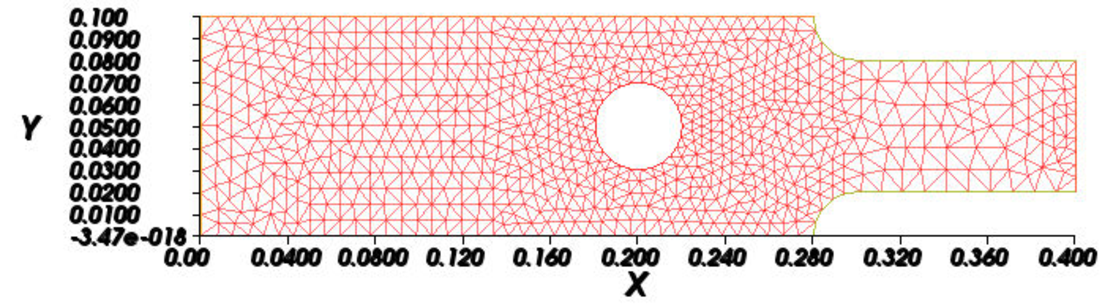
\includegraphics[width=1\textwidth]{paper/4-2-1.pdf}
\caption{Trạng thái ban đầu của tấm kim loại.}
\label{fig:exam21}
\end{figure}\\
Hình dưới đây cho thấy sự biến dạng của tấm kim loại chịu một lực kéo $F = 100$. Do lực kéo là rất nhỏ nên độ biến dạng của tấm kim loại là không lớn \eqref{fig:exam22}.\\
\begin{figure}[http]
\centering
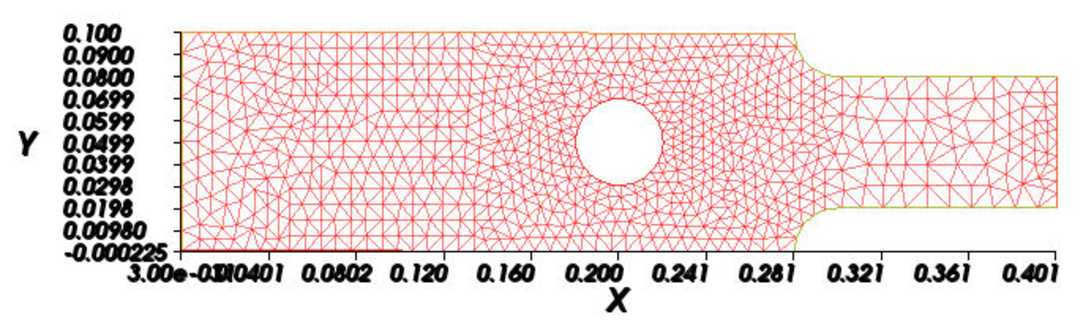
\includegraphics[width=1\textwidth]{paper/4-2-2.pdf}
\caption{Tấm kim loại dưới tác dụng của lực kéo F=100.}
\label{fig:exam22}
\end{figure}\\
Khi ta tăng lực kéo F lên F=5e3 (hình \ref{fig:exam23}) và F=1e4 (hình \ref{fig:exam24}) thì ta thấy độ biến dạng rõ hơn.\\
\begin{figure}[http]
\centering
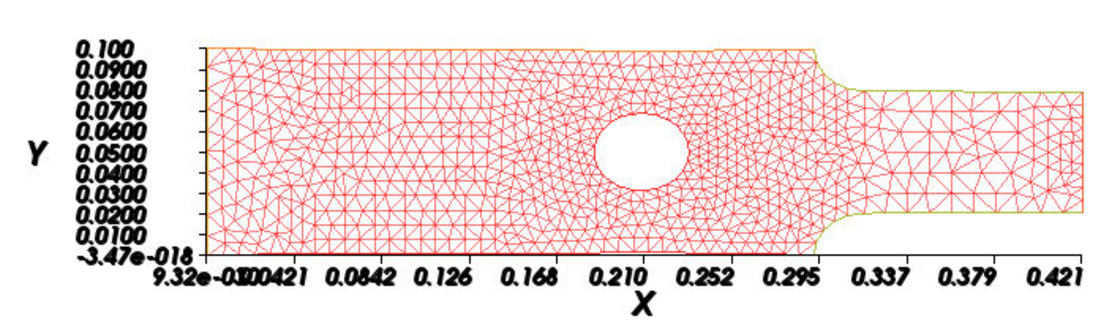
\includegraphics[width=1\textwidth]{paper/4-2-3.pdf}
\caption{Tấm kim loại dưới tác dụng của lực kéo F=5e3.}
\label{fig:exam23}
\end{figure}
\begin{figure}[http]
\centering
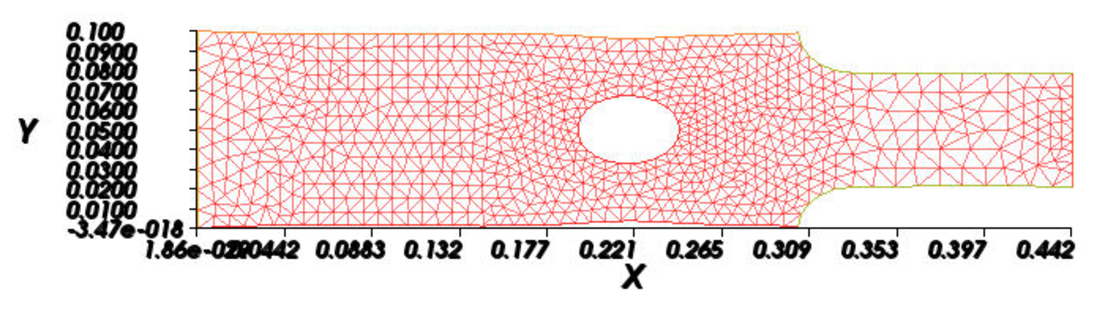
\includegraphics[width=1\textwidth]{paper/4-2-4.pdf}
\caption{Tấm kim loại dưới tác dụng của lực kéo F=1e4.}
\label{fig:exam24}
\end{figure}
\subsection{Lực nén}
Xét một tấm kim loại có một lỗ ở giữa chịu tác động của một lực nén $f=(-1e4,0)$ và trọng lực $g=(0,-9.81)$. Cho hằng số mô-đun đàn hồi Young $E=7e4$ và hệ số Poisson $v=0,3$ \cite{TIT-07}. Ta có hình \eqref{fig:exam31} - khởi tạo lưới ban đầu của tấm kim loại và hình \eqref{fig:exam32} - thể hiện lưới biến dạng của tấm kim loại sau khi chịu tác động bởi lực nén.\\
\begin{figure}[http]
\centering
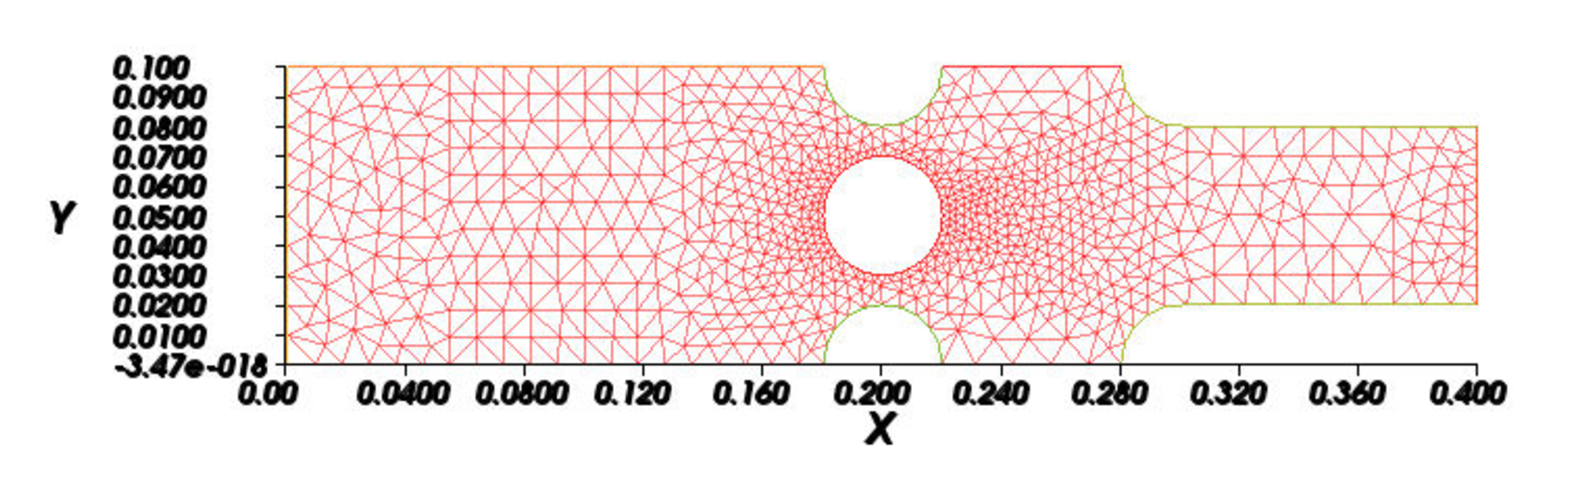
\includegraphics[width=1\textwidth]{paper/4-3-1.pdf}
\caption{Tấm kim loại ở trạng thái ban đầu.}
\label{fig:exam31}
\end{figure}
\begin{figure}[http]
\centering
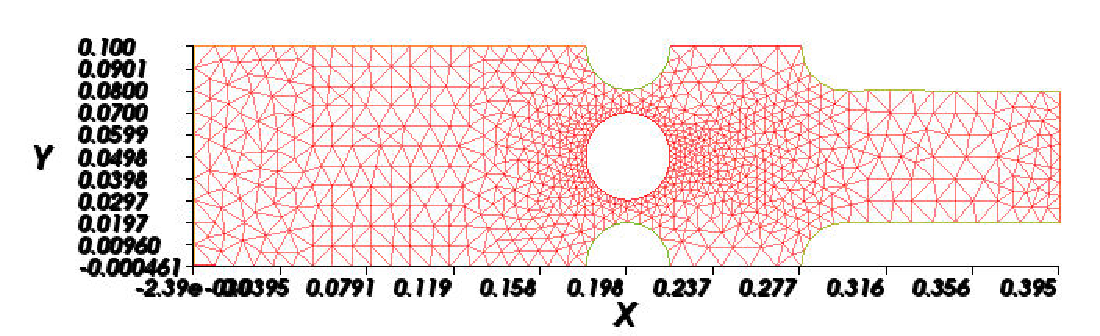
\includegraphics[width=1\textwidth]{paper/4-3-2.pdf}
\caption{Tấm kim loại dưới tác dụng của lực nén.}
\label{fig:exam32}
\end{figure}\\

Xét một tấm kim loại có kích thước là $2 * 2$ với đáy cố định, chịu tác dụng của một lực nén $f = 1e7$ lên phía trên của tấm kim loại. Tấm kim loại có một lỗ được cho bởi phương trình $r = 0.5 + 0.2 sin(kt)$ trong tọa độ cực. Trong ví dụ này, ta xét $k=5$. Cho hằng số mô-đun đàn hồi Young và hệ số Poisson lần lượt bằng $E=1e9, v=0,3$. Dưới đây là lưới khởi tạo với 5796 tam giác của tấm kim loại \ref{fig:exam33}:\\

\begin{figure}[http]
\centering
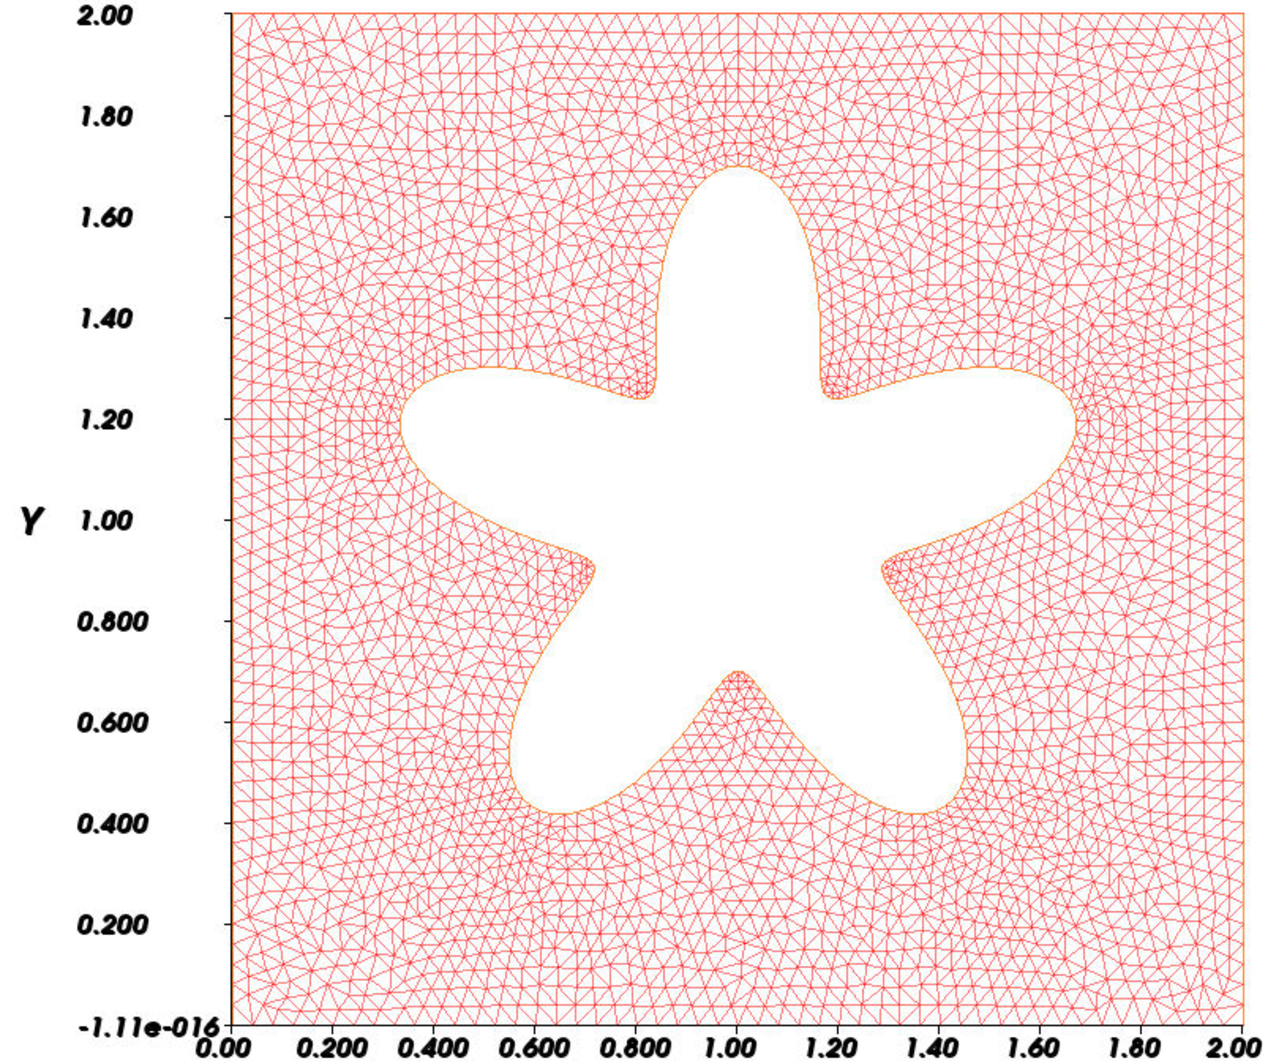
\includegraphics[width=0.6\textwidth]{paper/4-3-3.pdf}
\caption{Tấm kim loại $2 * 2$ với lỗ $r = 0.5 + 0.2 sin(kt)$.}
\label{fig:exam33}
\end{figure}
Dưới tác dụng của lực nén, tấm sẽ bị nén theo chiều y và phình to ra theo hướng x. Hình sau biểu thị sự dịch chuyển biến dạng của tấm kim loại:\\
\begin{figure}[http]
\centering
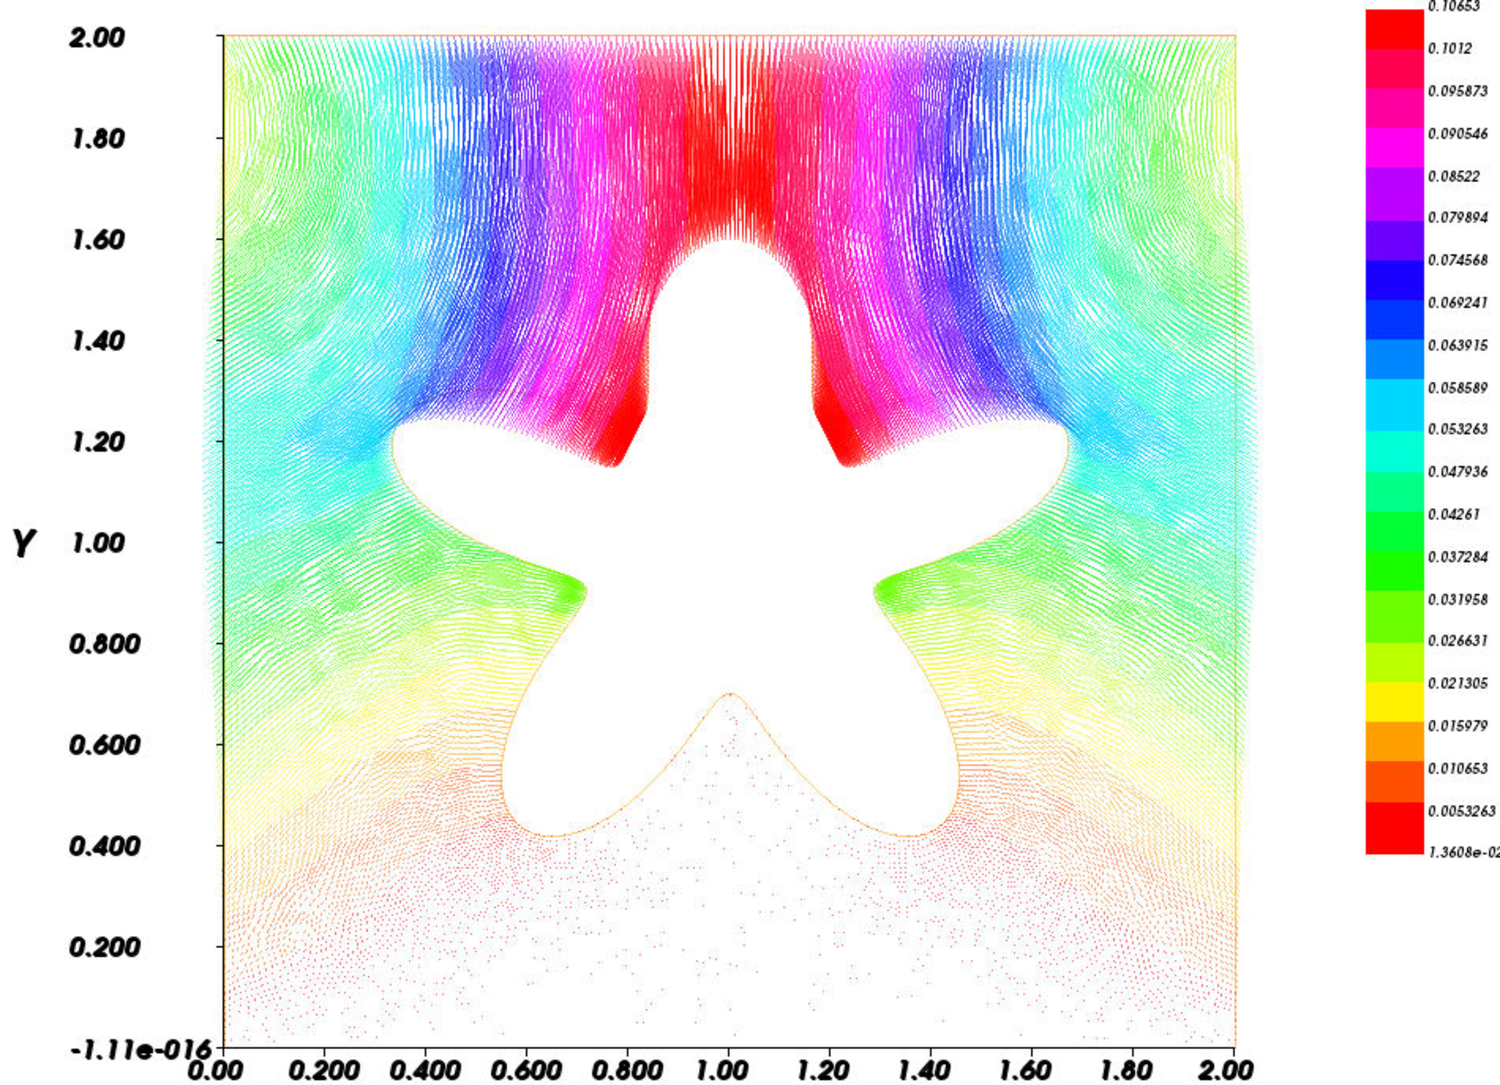
\includegraphics[width=0.6\textwidth]{paper/4-3-4.pdf}
\caption{Hướng dịch chuyển của tấm kim loại.}
\label{fig:exam34}
\end{figure}\\
\begin{figure}[http]
\centering
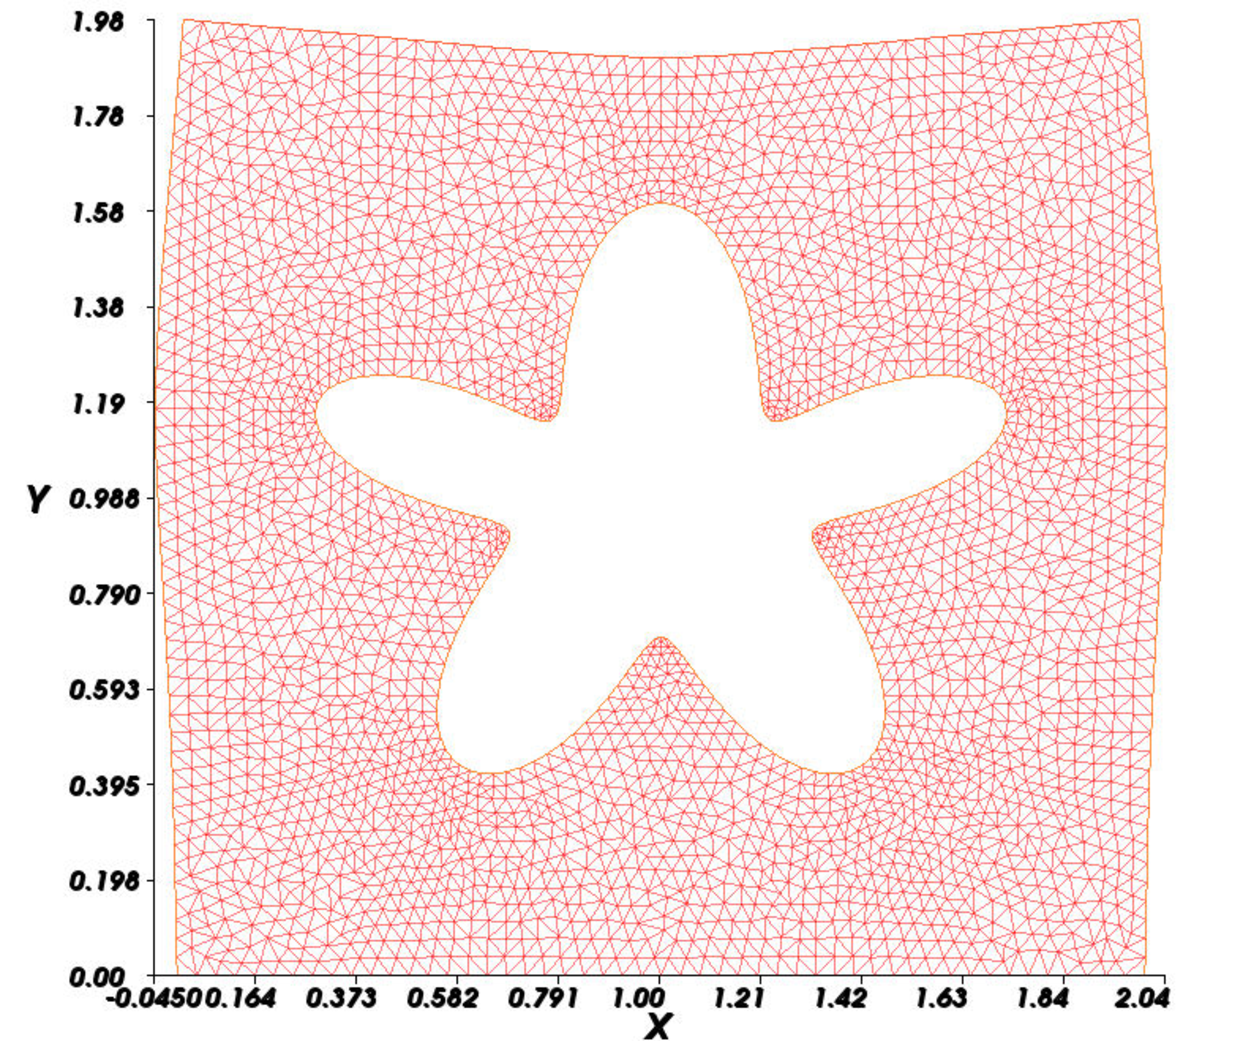
\includegraphics[width=0.6\textwidth]{paper/4-3-5.pdf}
\caption{Tấm kim loại sau khi bị biến dạng.}
\label{fig:exam35}
\end{figure}\\
\subsection{Áp suất}
Một tấm kim loại hình khuyên phải chịu một áp lực bên trong như hình \ref{fig:exam41} với $p=1e3,E=2e5, v=0.3, r_i=42, r_e=50, h=1 (h<<r_i)$ \cite{TIT-07}. Do $(h<<r_i)$ nên ta có thể coi đây là một bài toán 2 chiều. Ở ví dụ tiếp theo, ta xét một ống kim loại có cùng $p, E, v, r_i, r_e$ với chiều dài không nhỏ hơn quá nhiều so với bán kính của ống. Khi đó, bài toán trở thành bài toán 3 chiều.\\
\begin{figure}[http]
\centering
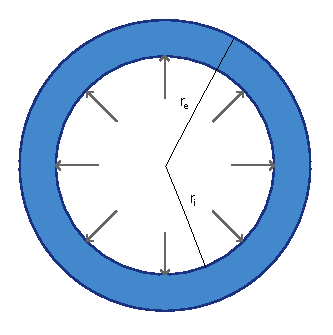
\includegraphics[width=0.5\textwidth]{paper/4-4.pdf}
\caption{Khuyên kim loại chịu tác động của áp suất ở bên trong.}
\label{fig:exam40}
\end{figure}\\
Sau đây là lưới khởi tạo với 1144 tam giác:\\
\begin{figure}[http]
\centering
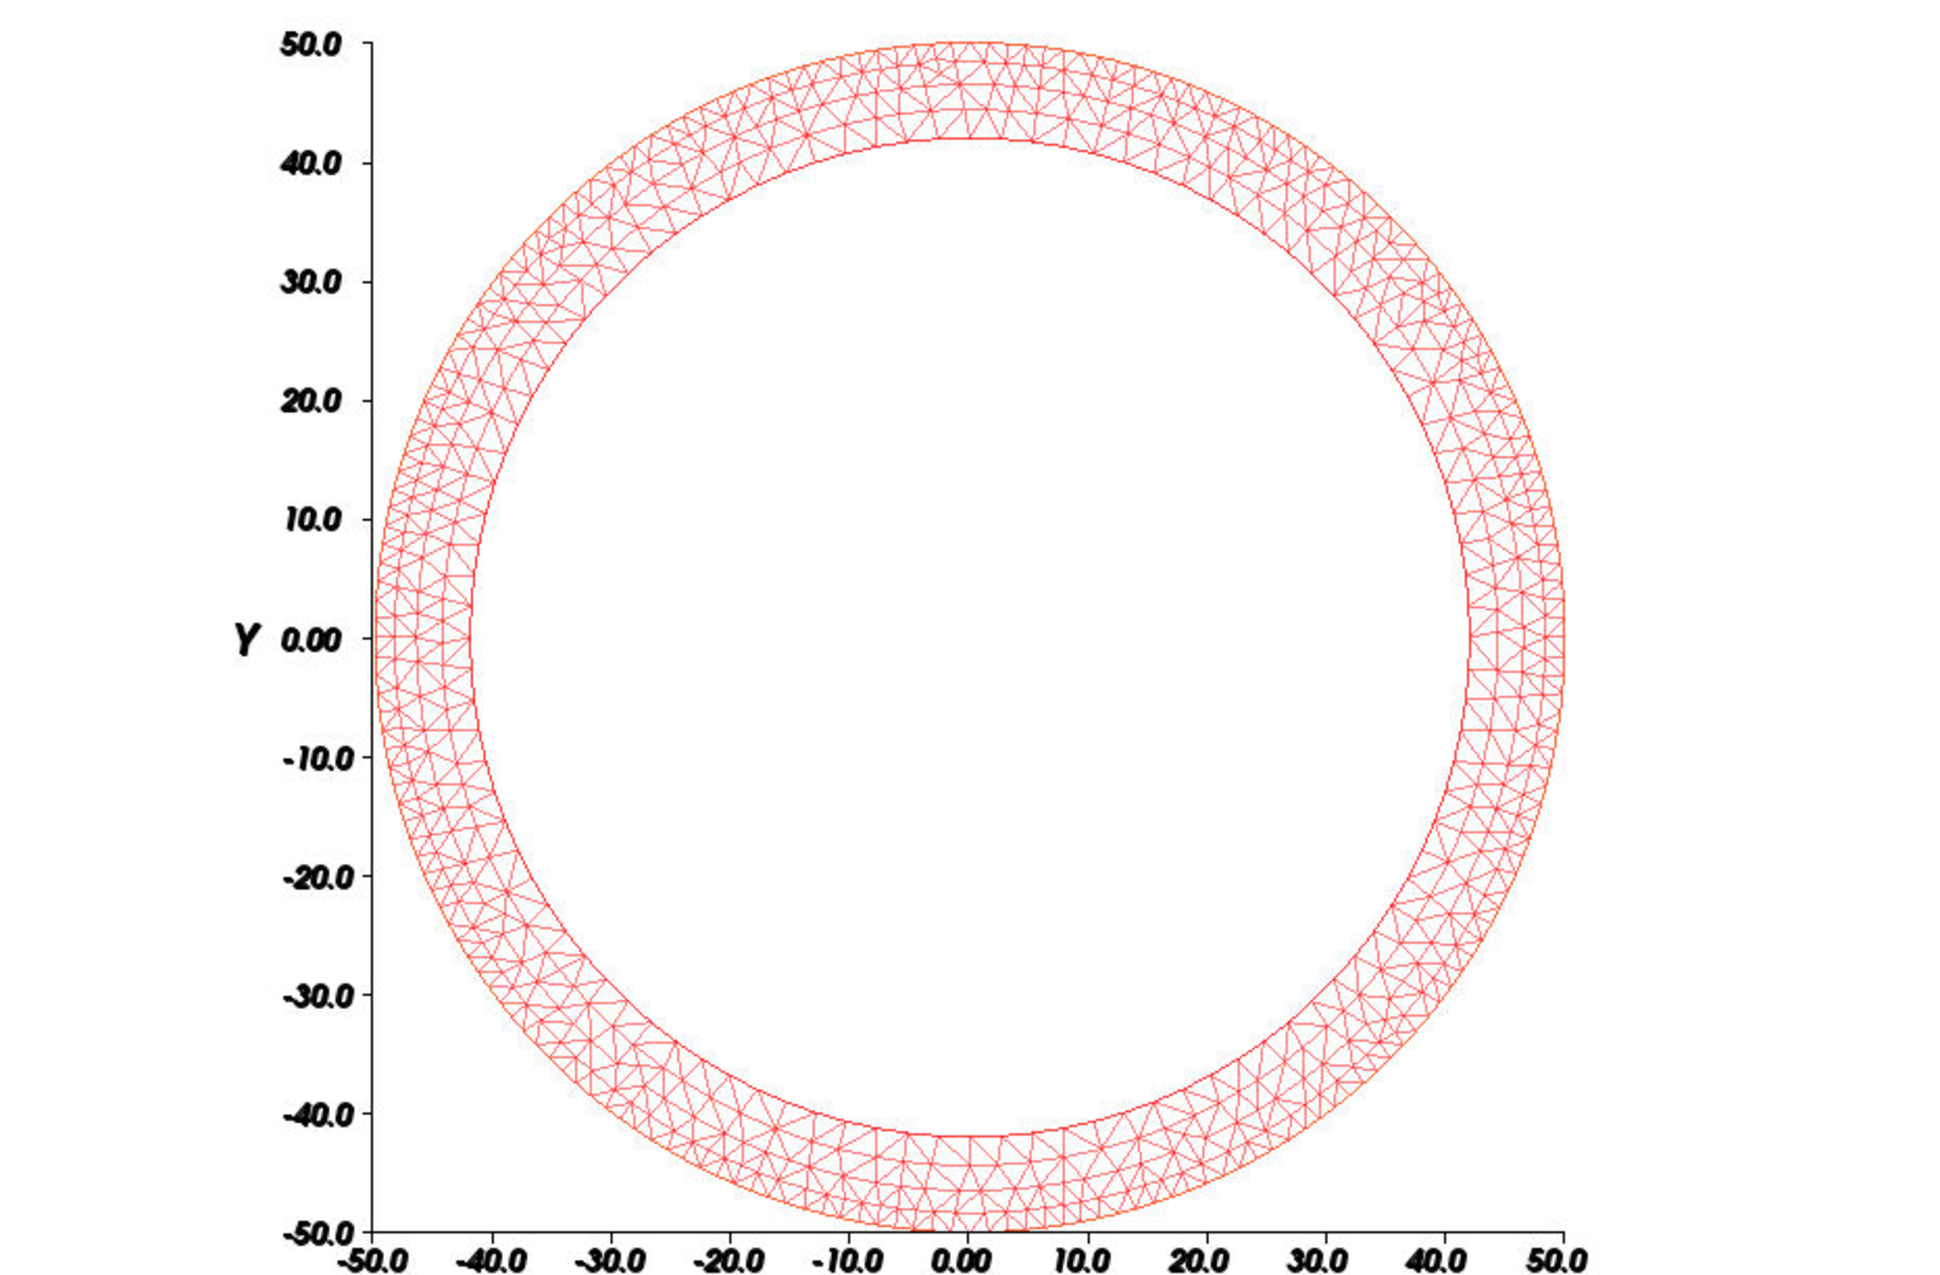
\includegraphics[width=0.7\textwidth]{paper/4-4-1.pdf}
\caption{Lưới khởi tạo của khuyên kim loại.}
\label{fig:exam41}
\end{figure}\\
Sự biến dạng của khuyên kim loại được biểu diễn như trong hình \ref{fig:exam42}:
\begin{figure}[http]
\centering
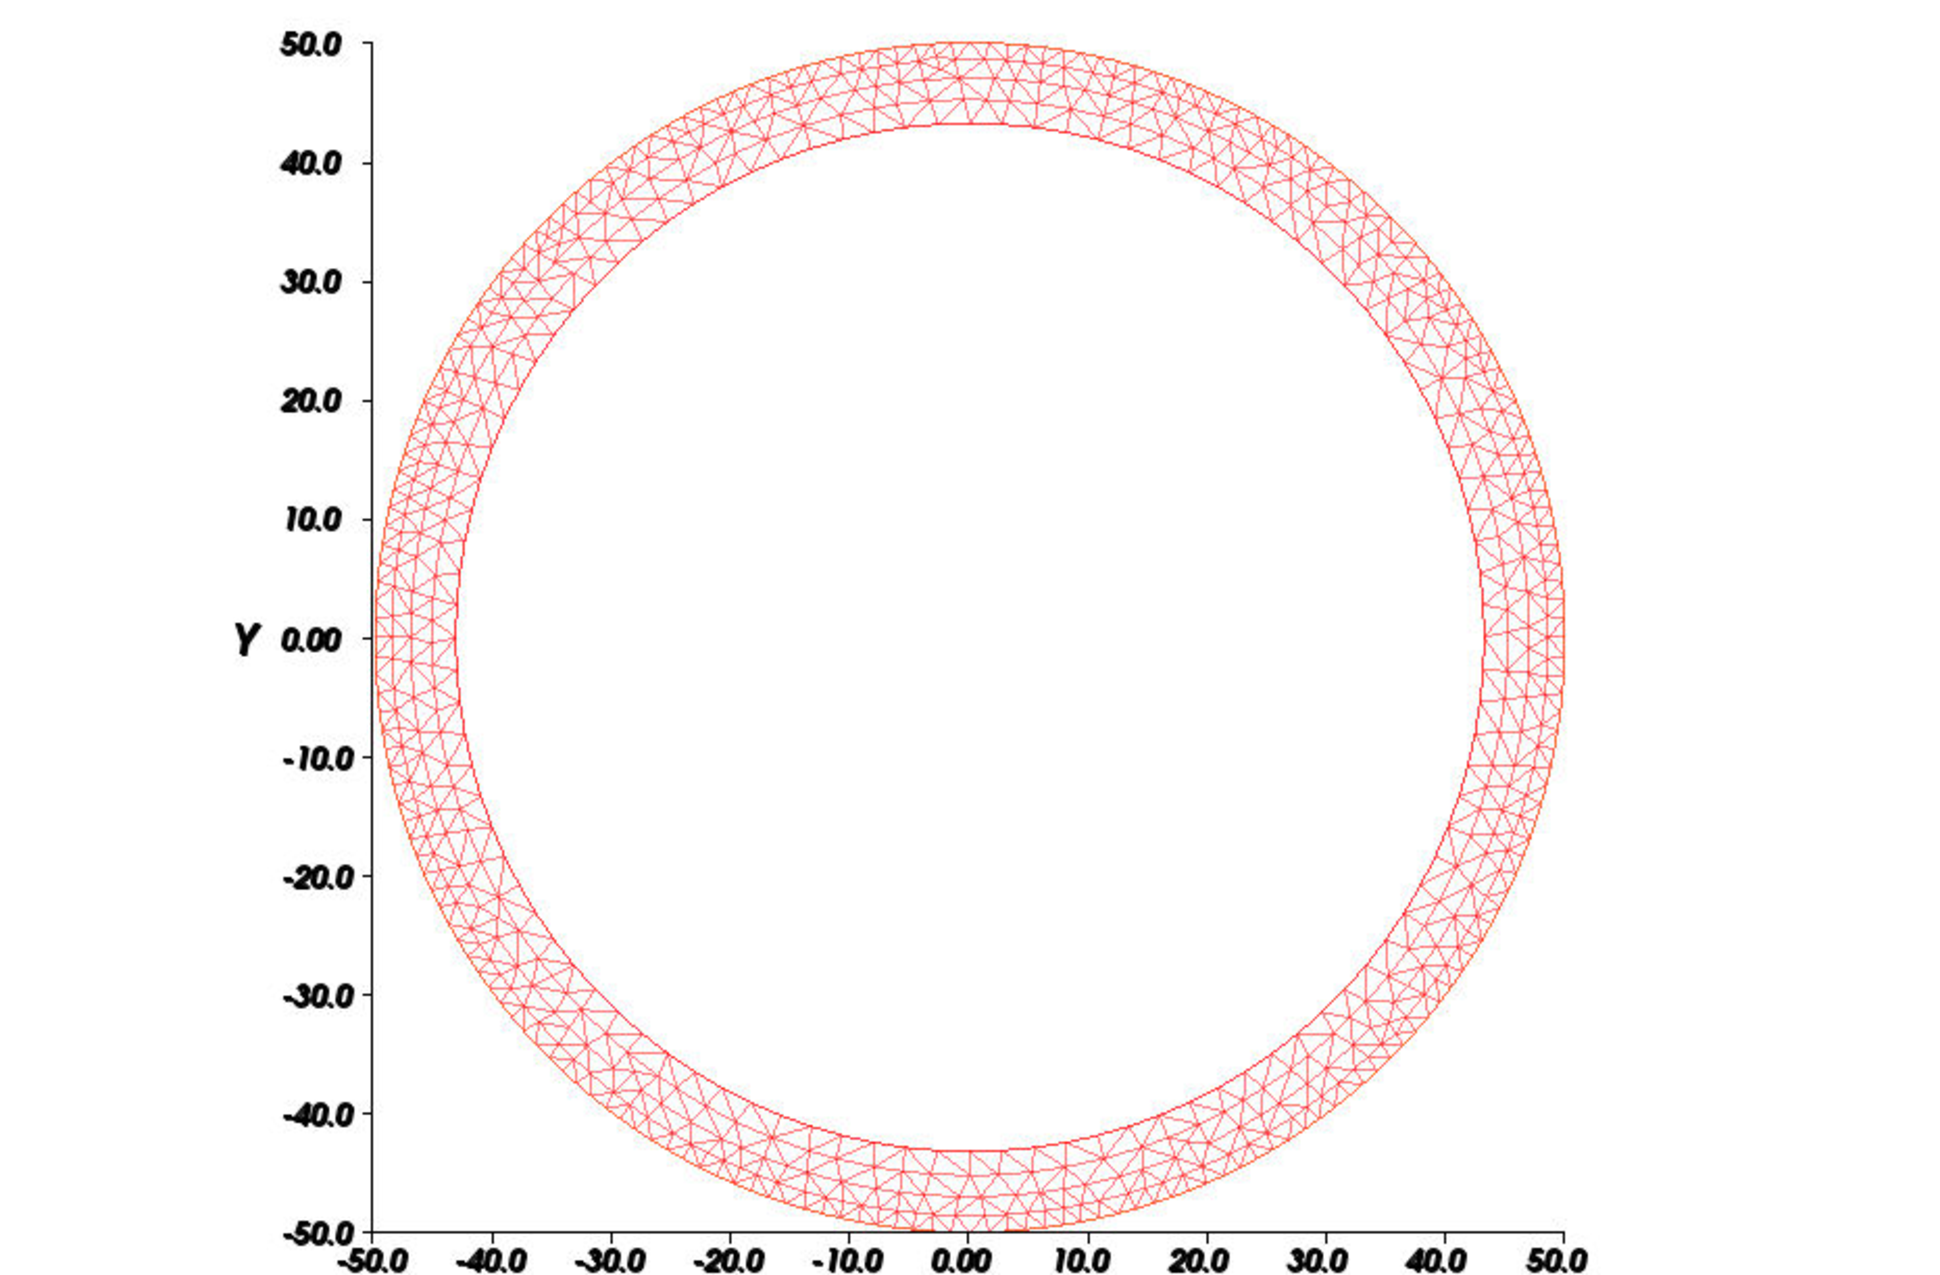
\includegraphics[width=0.7\textwidth]{paper/4-4-2.pdf}
\caption{Sự biến dạng của khuyên kim loại.}
\label{fig:exam42}
\end{figure}\\
Như đã nói ở trên, ta xét một ống kim loại. Có áp suất bên trong ống $p=1e3,E=2e5, v=0.3, r_i=40, r_e=50$ và ống có chiều dài $h=40$.\\
\begin{figure}[http]
\centering
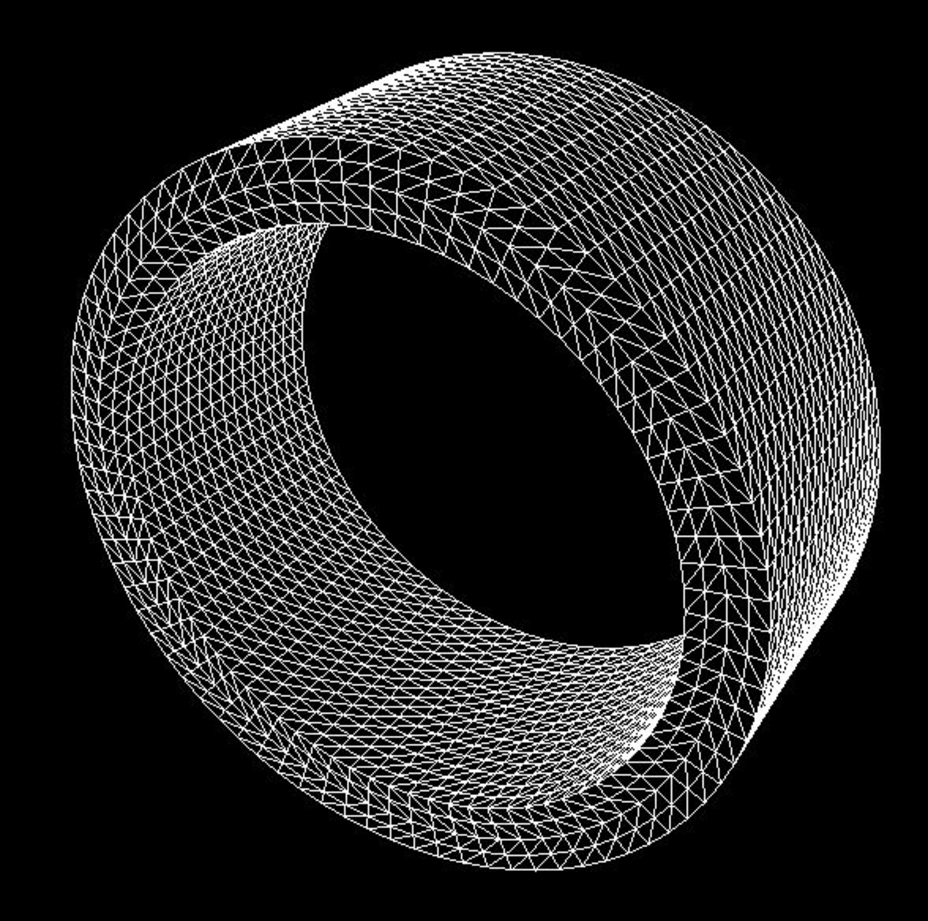
\includegraphics[width=0.6\textwidth]{paper/4-5.pdf}
\caption{Lưới khởi tạo của ống kim loại.}
\label{fig:exam50}
\end{figure}\\
Và các hình dưới đây cho thấy sự biến dạng của ống kim loại:
\begin{figure}[http]
\centering
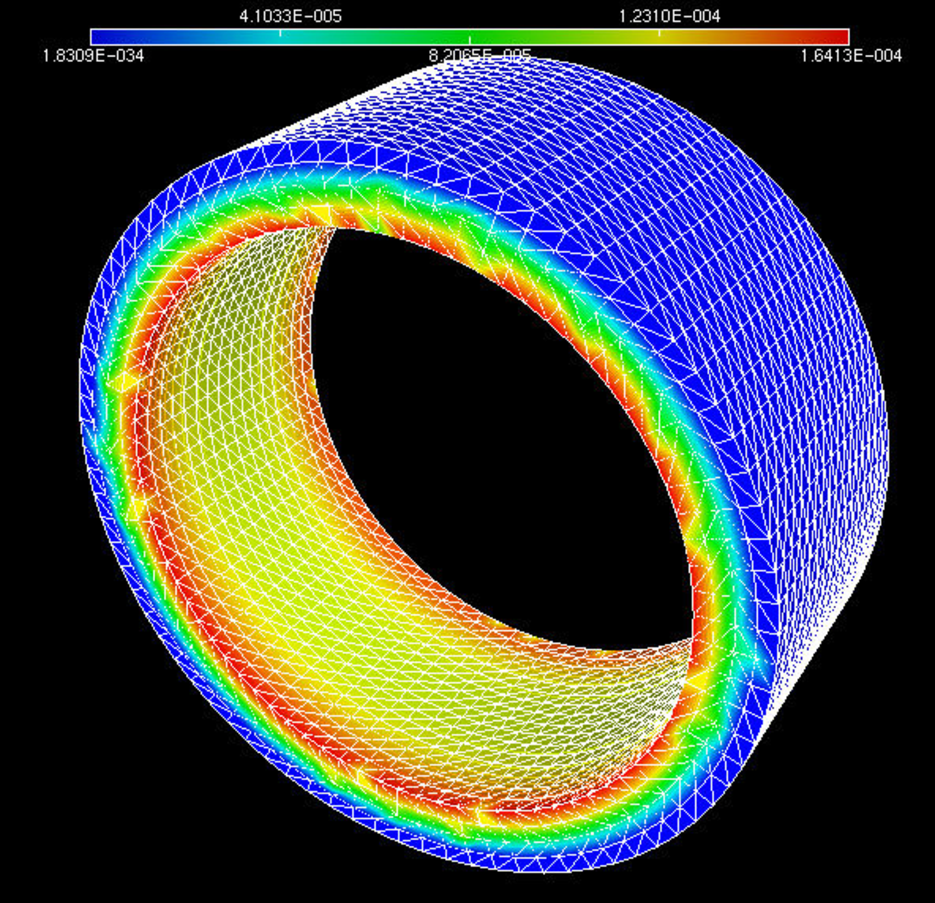
\includegraphics[width=0.6\textwidth]{paper/4-5-1.pdf}
\caption{Ống kim loại trước khi bị biến dạng.}
\label{fig:exam51}
\end{figure}\\
\begin{figure}[http]
\centering
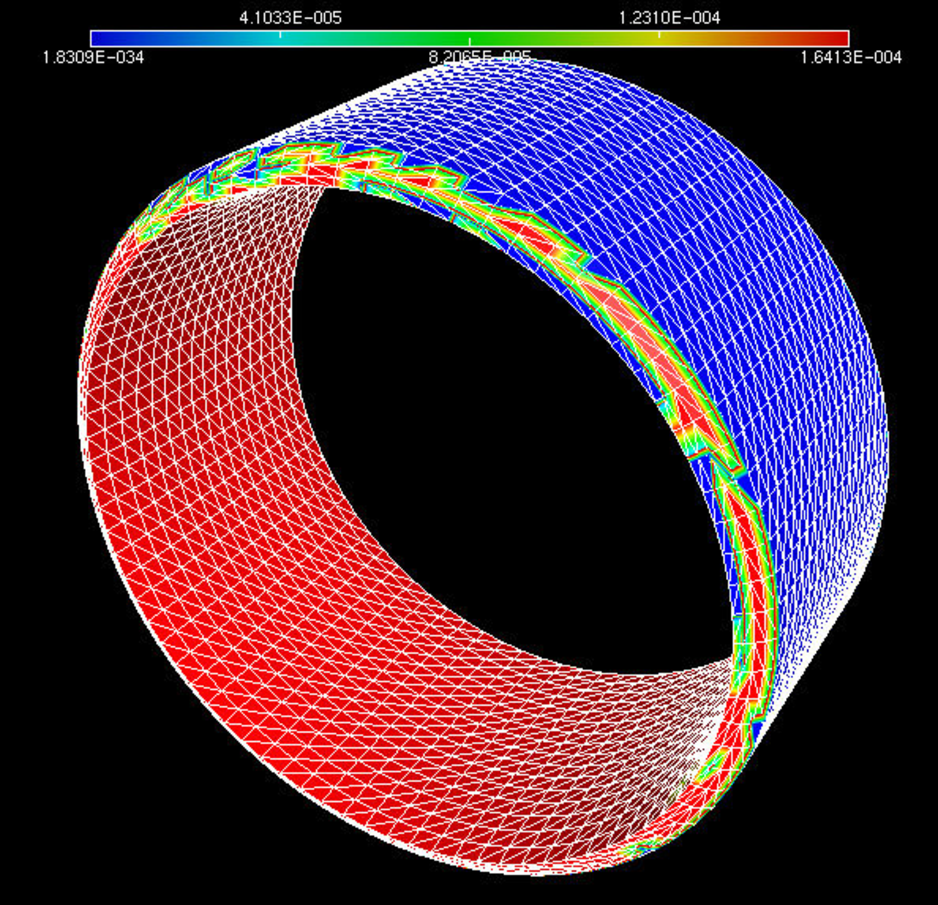
\includegraphics[width=0.6\textwidth]{paper/4-5-2.pdf}
\caption{Ống kim loại sau khi bị biến dạng.}
\label{fig:exam52}
\end{figure}\\

\section{Kết luận}
Trong chương này, ta đã trình bày chi tiết các bước xây dựng lược đồ giải số cho hệ phương trình biến dạng đàn hồi. Cụ thể, nội dung chương \ref{Chapter1} đã giải quyết những vấn đề sau:
\begin{itemize}
\item Phát biểu bài toán biến dạng đàn hồi.
\item Áp dụng phương pháp phần tử hữu hạn rời rạc hóa không gian, từ đó xây dựng bài toán rời rạc và hệ phương trình đại số tương ứng.
\item Trình bày các ví dụ giải số minh họa.
\end{itemize}

%----------------------------------------------------------------------------------------

% Chapter 1
\chapter{Kiến thức chuẩn bị}
\section{Không gian Hilbert}

\begin{defi}
Trong không gian có tích vô hướng $V$, ta xét chuẩn $||u||_V = \sqrt{(u,u)}$. Khi đó không gian vectơ $V$ là một không gian định chuẩn. Không gian định chuẩn này được gọi là không gian tiền Hilbert.\\
Không gian Hilbert là không gian tiền Hilbert đầy đủ.
\end{defi}
\subsubsection*{Một số không gian hàm}
Cho $\Omega \subset\mathbb{R}^n$ bị chặn.\\
$C(\overline{\Omega})$ là không gian các hàm liên tục trên $\overline{\Omega}$ với
$$||u||_{C(\overline{\Omega})}=\max_{x\in \overline{\Omega}}|u(x)|$$
Không gian $C^m(\overline{\Omega}) = \{u|D^\alpha u(x)\in C(\overline{\Omega}), \forall \alpha \leq m\}$\\
Trong đó $\alpha =(\alpha_1,\alpha_2,...,\alpha_n), \qquad |\alpha| = \alpha_1 + \alpha_2 + ... + \alpha_n.$
$$D^\alpha u(x)=\frac{\partial^{|\alpha|}u}{\partial^{\alpha_1}_{x_1}\partial^{\alpha_2}_{x_2}...\partial^{\alpha_n}_{x_n}}$$
\textbf{Không gian các hàm bình phương khả tích} $L_2(\Omega),\Omega \subset \mathbb{R}^n$
$$u \in L_2(\Omega)\Leftrightarrow\int_\Omega u^2(x)dx< +\infty ,\quad dx = dx_1dx_2...dx_n.$$
Tích vô hướng trong không gian $L_2(\Omega): u,v \in L_2(\Omega)$
$$(u,v)_{L_2(\Omega)}=(u,v)_\Omega=\int_\Omega u(x)v(x)dx.$$
Chuẩn trong không gian $L_2(\Omega)$:
$$||u||_{L_2(\Omega)}=\sqrt{(u,u)_{L_2(\Omega)}}=\sqrt{\int_\Omega u^2(x)dx}$$
Không gian các hàm bình phương khả tích $L_2(\Omega)$ là một không gian Hilbert.\\
\textbf{Không gian Sobolev}: $W^m_p(\Omega)$\\
Giả sử $m$ là một số nguyên không âm và miền $\Omega$ bị chặn, ta định nghĩa:
$$W^m_p(\Omega)=\{u|D^\alpha u(x)\in L_p(\Omega)\forall |\alpha|\leq m\}$$
Với $p=2$ thì ta có không gian $H^m(\Omega)$.
\textbf{Tích vô hướng:}
$$u,v\in H^m(\Omega)\quad (u,v)_{H^m(\Omega)}=\sum_{|\alpha|=0}^m(D^\alpha_u,D^\alpha_v)_{L_2(\Omega)}$$
\textbf{Chuẩn:}
$$||u||_{H^m(\Omega)}=\sqrt{(u,v)_{H^m(\Omega)}}$$
Đặc biệt với $m=1$
$$H^1(\Omega)=\{u\in L_2(\Omega)|Du\in L_2(\Omega)\}$$
$$||u||^2_{H^1(\Omega)}=\int_\Omega (u^2+\sum_{k=1}^mu^2_{x_k})dx$$
$$||u||^2_{H^1(\Omega)}=||u||^2_{L_2(\Omega)}+||Du||_{L_2(\Omega)}$$
Ký hiệu: $||.||_{H^m(\Omega)}=||.||_m$\\
\textbf{Giá của hàm số} $u(x), x\in\Omega\subset\mathbb{R}^n$
$$\text{supp}(u)=\overline{\{x|u(x)\neq 0\}}$$
$D(\Omega)$ là không gian các hàm khả vi vô hạn và có giá compact.\\
\textbf{Phiếm hàm:} Cho $V$ là một không gian Hilbert. $f$ là một phiếm hàm trên $V$ nếu $f$ là một ánh xạ từ $V$ vào $\mathbb{R}$ hay $f:V\rightarrow\mathbb{R}$.\\
Phiếm hàm $f$ là tuyến tính nếu: $f(\alpha u+\beta v)=\alpha f(u)+\beta f(v) \quad \forall u,v\in V;\forall \alpha,\beta \in \mathbb{R}$.\\
Phiếm hàm $f$ liên tục nếu: $\exists c>0:|f(v)|\leq c||v||_V \forall v\in V$\\
\textbf{Dạng song tuyến tính:} Cho $V$ là một không gian Hilbert. $a(u,v)$ là một dạng song tuyến tính trên $V$ nếu nó là một ánh xạ từ $V\times V$ vào $\mathbb{R}$ hay $a(.,.):V\times V\rightarrow \mathbb{R}$ thỏa mãn:
$$a(u, \alpha v_1+\beta v_2) = \alpha a(u,v_1)+\beta a(u,v_2)$$
$$a(\alpha u_1+\beta u_2,v) = \alpha a(u_1,v)+\beta a(u_2,v)$$
$a(.,.)$ được gọi là đối xứng nếu $a(u,v)=a(v,u) \quad \forall u,v\in V$.\\
$a(.,.)$ bị chặn hay liên tục nếu $\exists c_1>0$ sao cho $|a(u,v)|\leq c_1||u||_V||v||_V$\\
$a(.,.)$ được gọi là V-elliptic nếu $\exists c_2>0$ sao cho $a(u,u)\geq c_2||u||_V\quad\forall u\in V$
\section{Bài toán yếu trong không gian Hilbert}
\subsubsection*{Bài toán yếu}
Xét không gian Hilbert $V$. Cho $a(u,v)$ là một dạng song tuyến tính trên $V$, $L(v)$ là một phiếm hàm tuyến tính trên $V$. Bài toán: Tìm $u\in V$ thỏa mãn
\begin{equation}\label{eq:bty}
a(u,v) = L(v), \qquad \forall v\in V
\end{equation}
gọi là bài toán yếu trong không gian Hilbert.
\subsubsection*{Dạng biến phân của bài toán yếu}
\begin{lem}
Nếu dạng song tuyến tính $a(u,v)$ đối xứng, liên tục trên $V$ và V-eliptic, đồng thời phiếm hàm tuyến tính $L(v)$ liên tục trên $V$ thì bài toán yếu \ref{eq:bty} tương đương với bài toán
\begin{equation}\label{eq:btmin}
J(u)=\min_{v\in V} J(u)
\end{equation}
Trong đó: $J(u) = a(v,v)-2L(v),\qquad\forall v\in V.$
\end{lem}
Bài toán \ref{eq:btmin} được gọi là dạng biến phân của bài toán yếu \eqref{eq:bty}.\\
\textit{Chứng minh:} Cho $t\in \mathbb{R}$
$$J(u+tv)=a(u+tv,u+tv)-2L(u+tv)$$
$$= a(u,u)-2L(u)+2t[a(u,v)-L(v)]+t^2a(v,v)$$
Do $J(u) = a(v,v)-2L(v)$ nên
$$\Rightarrow J(u+tv)-J(u)=2t[a(u,v)-L(v)]+t^2a(v,v)$$
Nếu $u$ là nghiệm của bài toán yếu \ref{eq:bty} thì
$$J(u+tv)-J(u)=t^2a(v,v)\geq 0,\forall t\in\mathbb{R},\forall v\in V$$
$$\Rightarrow u=\text{argmin}_{v\in V}J(v)$$
Vậy $u$ là nghiệm của bài toán biến phân \ref{eq:btmin}.
Nếu $u$ là nghiệm của bài toán biến phân \ref{eq:btmin} thì
$$u=\text{argmin}_{v\in V}J(v) \Rightarrow J(u+tv)-J(u)\geq 0,\forall t\in\mathbb{R},\forall v\in V$$
$$\Rightarrow 2t[a(u,v)-L(v)]+t^2a(v,v)\geq 0 ,\forall t\in\mathbb{R},\forall v\in V$$
$$\Leftrightarrow a(u,v)-L(v)=0 \forall v\in V.$$
Vậy $u$ là nghiệm của bài toán yếu \ref{eq:bty}.
\subsubsection*{Sự tồn tại nghiệm của bài toán yếu}
\begin{thm}[Định lý Lax-Milgram]\label{thm:LM}
Cho $a(.,.)$ là dạng song tuyến tính bị chặn trên $V$ và là V-elliptic. $L(.)$ là phiếm hàm tuyến tính bị chặn trên $V$. Khi đó bài toán yếu \ref{prowf} có nghiệm và nghiệm đó là duy nhất.
\end{thm}
%\textit{Chứng minh}
\chapter{Giải bài toán biến dạng đàn hồi bằng phương pháp phần tử hữu hạn}\label{Chapter1}
\renewcommand{\baselinestretch}{1.25}
\minitoc
\renewcommand{\baselinestretch}{1.5}
Trong chương này, ta sẽ trình bày một lược đồ giải số cho bài toán biến dạng đàn hồi. Phần đầu tiên, một vài kiến thức cơ sở. Phần \ref{sec:chap1_problem} phát biểu phương trình biến dạng đàn hồi. Phần \ref{sec:chap1_characteristicMethod} dẫn dắt đưa bài toán ban đầu về dưới dạng biến phân. Phương pháp phần tử hữu hạn sẽ được sử dụng để rời rạc hóa không gian trong phần \ref{sec:chap1_spatialDiscrete}. Phần tiếp theo \ref{sec:chap1_linearSystem} trình bày cách xây dựng hệ phương trình tuyến tính rời rạc. Và cuối cùng là một vài ví dụ của bài toán trong công nghiệp vật liệu.

%----------------------------------------------------------------------------------------

\section{Phương trình đàn hồi}\label{sec:chap1_problem}
Cho $\Om$ là miền trong không gian $\R^d (d=2 \text{ hoặc } 3)$ có biên $\Gamma = \{\Gamma_D, \Gamma_N\}$. $\Gamma_D$ là điều kiện biên Dirichlet, $\Gamma_N$ là điều kiện biên Neumann. Gọi u là dịch chuyển biến dạng của một tấm được cấu tạo vật liệu khác nhau. Mối quan hệ giữa biến dạng và dịch chuyển biến dạng của tấm được đưa ra: % ????
$$e(u) = (\nabla u + \nabla u^t)/2$$

Giả sử rằng vật liệu có tính đàn hồi tuyến tính và đẳng hướng; và rằng các dịch chuyển biến dạng là không quá lớn gây ra sự mất cấu trúc của vật, định luật Hooke đưa ra mối quan hệ giữa ứng suất và biến dạng:
\begin{equation}\label{equa1}
\mathcal{A}e(u) = 2\mu e(u) + \lambda Tr(e(u))Id
\end{equation}
trong đó:
\begin{itemize}
\item $\mathcal{A}e(u)$ là ứng suất,
\item $Id$ là ma trận đơn vị,
\item $Tr(.)$ là vết của hàm,
\item $\lambda, \mu$ là các hệ số Lamé mô tả các tính chất cơ học của vật. Do sự ổn định của phương trình nhiệt động lực học, các hệ số này thỏa mãn các điều kiện sau: $\mu >0$ và $\lambda + \frac{2}{3}\mu \geq 0$ \cite{AJT04}. Hơn nữa, để giảm độ phức tạp của bài toán, ta giả sử rằng $\lambda ,\mu$ là hằng số sao cho  $\lambda \geq 0$.
\end{itemize}
\begin{rem}
$\quad$
\begin{enumerate}{\roman{enumii}}
\item Hệ số $\lambda + \frac{2}{3}\mu$ mô tả khả năng biến  của vật, giá trị của hệ số này càng lớn thì tương đương với việc vật liệu gần như không thể nén.
\item Thay vì sử dụng hệ số Lamé $\lambda$ và $\mu$, ta thường sử dụng các hằng số được biết đến nhiều hơn, một phần cũng là để thuận tiện hơn. Đó là hằng số mô-đun đàn hồi Young $E$ và hệ số Poisson $\nu$. Ta có mối quan hệ giữa các hằng số này được biểu diễn như sau:
$$E = \mu \frac{3\lambda +2\mu}{\lambda +\mu}, \qquad \nu=\frac{1}{2}\frac{\lambda}{\lambda +\mu}$$
hay
$$\mu = \frac{E}{2(1 + \nu)}, \qquad \lambda = \frac{E\nu}{(1 + \nu)(1 - 2\nu)}.$$
Hệ số Poisson thỏa mãn $-1\leq \nu\leq \frac{1}{2}$. Do ta giả sử $\lambda \geq 0$ nên $\nu\geq 0$. Một vật liệu gần như không thể nén thì tương ứng với nó là hệ số Poisson xấp xỉ bằng $\frac{1}{2}$.
\item Mô hình đàn hồi đẳng hướng tuyến tính nói chung được áp dụng vào trong các bài toán biến dạng mà trong đó độ biến dạng của vật liệu là rất nhỏ. Trong trường hợp này, để cho đơn giản thì các lực tác động lên vật đều là tuyến tính.
\end{enumerate}
\end{rem}
Gọi $g$ là ngoại lực tác động bên ngoài, $f$ là trọng lực của vật. Ta thêm các điều kiện biên cho bài toán đàn hồi. Từ đó, ta được hệ phương trình tuyến tính đàn hồi:
\begin{equation}\label{prob}
\quad\quad\quad\quad\quad
\begin{cases}
-\text{div}(\mathcal{A}e(u)) = f \qquad \text{trong } \Omega,\\
u = 0 \quad\qquad\qquad\qquad \text{trên } \Gamma_D, \\
\mathcal{A}e(u))n = g \qquad\qquad \text{trên } \Gamma_N.
\end{cases}
\end{equation}

\section{Công thức biến phân}\label{sec:chap1_characteristicMethod}
Như đã thảo luận trong phần trước, việc biến đổi bài toán mô tả các vấn đề cơ học (strong form) về bài toán dạng yếu (weak form) hay bài toán biến phân là một bước quan trọng của phương pháp phần tử hữu hạn. Do đó, trong phần này, ta sẽ nghiên cứu dạng biến phân của hệ phương trình tuyến tính đàn hồi \eqref{prob}.\\

Ký hiệu $V$ là không gian hàm của dịch chuyển biến dạng $u$. Gọi $v \in V$ là hàm thử. Nhân cả hai vế phương trình đầu tiên của hệ \eqref{prob} với hàm thử $v$ rồi lấy tích phân trên miền $\Omega$, ta được:
$$-\int_\Omega\text{div}(\mathcal{A}e(u)).v = \int_\Omega f.v$$
Áp dụng công thức Green cho vế trái ta được:
$$\int_\Omega\mathcal{A}e(u).\nabla v - \int_{\partial \Omega}(\mathcal{A}e(u)n) = \int_\Omega f.v.v,$$
$$\int_\Omega\mathcal{A}e(u).\nabla v = \int_\Omega f.v + \int_{\partial \Omega}(\mathcal{A}e(u)n).v$$
Ta định nghĩa $a : b = \sum_{ij}{a_{ij}b_{ij}}.$ Không gian hàm thử $V$ được chọn sao cho hàm thử $v \in V$ bị triệt tiêu trên phần biên đặt điều kiện Dirichlet, nghĩa là:
$$V = H^1_{\Gamma_D}(\Omega)^d := \{v \in H^1(\Omega)^d : v = 0|\Gamma_D\}.$$
Kết hợp với điều kiện biên Neumann của hệ \eqref{prob}, ta có thể viết lại:
$$\int_\Omega\mathcal{A}e(u):e(v) = \int_\Omega f.v + \int_{\Gamma_N}g.v$$
Thay \eqref{equa1} vào ta được:
$$\int_\Omega(2\mu e(u) + \lambda Tr(e(u))Id):e(v) = \int_\Omega f.v + \int_{\Gamma_N}g.v$$
$$\int_\Omega 2\mu e(u) : e(v) + \lambda(\text{div}u)(\text{div}v) = \int_\Omega f.v + \int_{\Gamma_N}g.v.$$\\
Bài toán biến dạng đàn hồi có thể viết dưới dạng yếu tương đương: tìm $u\in V$ thỏa mãn:
\begin{equation}\label{prowf}
a(u,v) = L(v)
\end{equation}
Trong đó :
$$a(u,v) = \int_\Omega 2\mu e(u) : e(v) + \lambda(\text{div}u)(\text{div}v)$$
$$L(v) = \int_\Omega f.v + \int_{\Gamma_N}g.v$$
Sự tồn tại và duy nhất nghiệm của bài toán yếu \ref{prowf} của bài toán đàn hồi được chứng minh dựa theo định lý Lax-Milgram.
\section{Bài toán rời rạc của bài toán}
Thêm đánh giá sai số
Sử dụng xấp xỉ phần tử hữu hạn, không gian hàm thử $V$ được thay thế bằng một không gian con hữu hạn chiều $V_N$. Dạng rời rạc không gian tương ứng của bài toán \ref{prowf}: Tìm $u_h \in V_N$
sao cho $u_h = 0$ trên $\Gamma_D$ và với mọi $v_h \in V_N$ với $v_h = 0$ trên $\Gamma_D$,
\begin{equation}\label{prod}
\int_\Omega 2\mu e(u_h) : e(v_h) + \lambda(\text{div}u_h)(\text{div}v_h) = \int_\Omega f.v_h + \int_{\Gamma_N}g.v_h
\end{equation}
\section{Hệ phương trình tuyến tính}\label{sec:chap1_linearSystem}
Gọi $\mathcal{T}$ là tập các tam giác của $\Omega$ sau khi rời rạc hóa. Gọi $\mathcal{N}$ là tập tất cả các nút của $\mathcal{T}$; Tập $(\eta_k,...,\eta_{dN})=(\varphi_1e_1, \varphi_2e_2,...,\varphi_1e_d,...,\varphi_Ne_1,\varphi_Ne_2,...,\varphi_Ne_d)$ là tập các nút cơ sở của không gian con hữu hạn chiều $V_N$, trong đó $N$ tổng số đỉnh của lưới, $d$ là số chiều của vec-tơ chuyển vị, và $\varphi_i$ là hàm mũ tại đỉnh $x_i$ trong tam giác $\mathcal{T}$:
$$\varphi_{x_i}(x_j) = \begin{cases}
1 \text{ với } x_i = x_j, \\
0 \text{ với } x_i \neq x_j.
\end{cases}$$
Áp dụng điều kiện biên với $i = 1,...,dN$, ta được:
$$\int_\Omega 2\mu e(u_h) : e(\eta_i) + \lambda(\text{div}u_h)(\text{div}\eta_i) = \int_\Omega f.\eta_i + \int_{\Gamma_N}g.\eta_i.$$
Khi đó, véc-tơ chuyển vị được viết lại dưới dạng: $u_h = \sum_{j=1}^{dN}U_i\eta_i$. Từ đó ta có được hệ phương trình tuyến tính:
$$\displaystyle\sum^{dN}_{i=1}(\displaystyle\int_\Omega 2\mu e(\eta_j) : e(\eta_i) + \lambda(\text{div}\eta_j)(\text{div}\eta_i)) = \int_\Omega f.\eta_i + \int_{\Gamma_N}g.\eta_i.$$
Ký hiệu $A=(A_{ij})\in\mathbb{R}^{dN \times dN}$, trong đó:
$$A_{ij}=\displaystyle\int_\Omega 2\mu e(\eta_j) : e(\eta_i) + \lambda(\text{div}\eta_j)(\text{div}\eta_i),$$
Ma trận $A$ còn được gọi là ma trận độ cứng (stiffness matrix). Ký hiệu ma trận vế phải $B=(b_i)\in\mathbb{R}^{dN}$, trong đó:
$$b_i=\int_\Omega f.\eta_i + \int_{\Gamma_N}g.\eta_i.$$
Ta thu được hệ phương trình đại số tương ứng của bài toán đàn hồi \eqref{prob}:
\begin{equation}\label{pron}
Au=B
\end{equation}
Ma trận độ cứng $A$ là ma trận thưa, đối xứng và nửa xác định dương.
\section{Các ví dụ mô phỏng số}
Trong phần này, ta sẽ minh họa các ví dụ mô phỏng số cho hệ phương trình tuyến tính đàn hồi. Hầu hết các thí nghiệm sẽ được tiến hành trong không gian $d=$ hai chiều. Riêng ví dụ cuối là mô phỏng biến dạng trong $d=$ ba chiều.\\
Mã nguồn chương trình và một số thí nghiệm giải số cho các bài toán biến dạng đàn hồi có thể tìm thấy tại địa chỉ: \url{https://github.com/}. Tác giả luôn mong muốn nhận được những đề xuất, đóng góp cho việc phát triển mã nguồn và các thí nghiệm mô phỏng số.
\subsection{Thứ nguyên}
Nhiều thông số, phép đo trong khoa học vật lý và kỹ thuật được thể hiện dưới dạng một số cụ thể - một đại lượng số và một đơn vị tương ứng. Thông thường các đại lượng vật lý được thể hiện bằng các đơn vị thứ nguyên khác nhau; ví dụ, gia tốc trọng trường là sự kết hợp giữa chiều dài và thời gian, ví dụ. $9,81m/s^2$. Đôi khi đó là các đơn vị dẫn xuất. Ví dụ: một newton là $1 kg.m/s^2$. Bảy đại lương cơ sở và đơn vị tương ứng của chúng là: chiều dài (mét-m), khối lượng (kilôgam), thời gian (giây), cường độ dòng điện (ampere-A), nhiệt độ (Kelvin-K), lượng chất (mol-mol), cường độ sáng (candela-cd).\\
Trong bài toán đàn hồi, thông thường để hiển thị độ biến dạng được rõ hơn, ta thường thêm hệ số phóng đại. Trong tất cả ví dụ ở phần tiếp theo, tất cả các thông số vật lý đều được chuyển về cùng đơn vị và để cho đơn giản các đơn vị thứ nguyên đều được loại bỏ.
\begin{center}
\begin{tabular}{ |c|c|c| } 
 \hline
 Đại lượng vật lý & Ký hiệu & Đơn vị \\ 
 \hline
 Chiều dài, bán kính & $r_i, r_e, x, y$ & $m$ \\ 
 Hệ số đàn hồi Young & $E$ & $N/m^2$ \\ 
 Trọng lực & $g$ & $N$ \\ 
 Lực & $F$ & $N$ \\ 
 Áp suất & $p$ & $N/m^2$ \\ 
 \hline
\end{tabular}
\end{center}
\subsection{Mô phỏng thí nghiệm với lực kéo}
Trong phần này, ta sẽ trình bày các kết quả mô phỏng số cho bài toán liên quan đến lực kéo đàn hồi.\\
Cho một tấm kim loại có một lỗ ở giữa chịu lực kéo $F=(1e4,0)$ tại $x=0.4$ và trọng lực $g=(0,-9.81)$ với hằng số mô-đun đàn hồi Young $E=7e4$ và hệ số Poisson $v=0,3$ \cite{TIT-07}. Khởi tạo lưới với 1607 tam giác \eqref{fig:exam21}.\\
\begin{figure}[http]
\centering
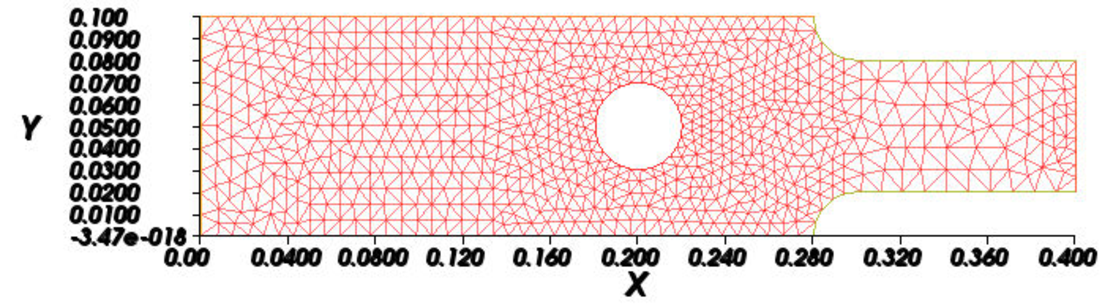
\includegraphics[width=1\textwidth]{paper/4-2-1.pdf}
\caption{Trạng thái ban đầu của tấm kim loại.}
\label{fig:exam21}
\end{figure}\\
Hình dưới đây cho thấy sự biến dạng của tấm kim loại chịu một lực kéo $F = 100$. Do lực kéo là rất nhỏ nên độ biến dạng của tấm kim loại là không lớn \eqref{fig:exam22}.\\
\begin{figure}[http]
\centering
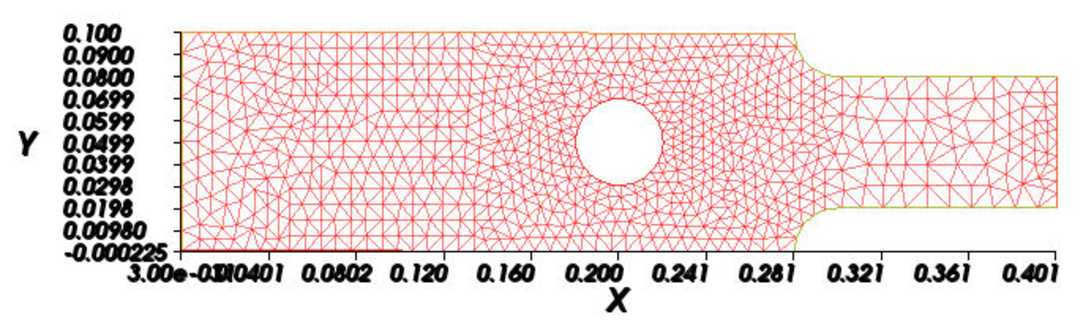
\includegraphics[width=1\textwidth]{paper/4-2-2.pdf}
\caption{Tấm kim loại dưới tác dụng của lực kéo F=100.}
\label{fig:exam22}
\end{figure}\\
Khi ta tăng lực kéo F lên F=5e3 (hình \ref{fig:exam23}) và F=1e4 (hình \ref{fig:exam24}) thì ta thấy độ biến dạng rõ hơn.\\
\begin{figure}[http]
\centering
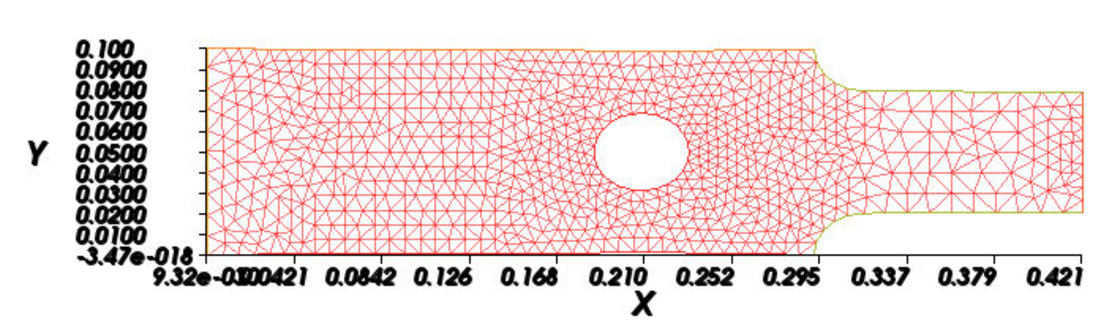
\includegraphics[width=1\textwidth]{paper/4-2-3.pdf}
\caption{Tấm kim loại dưới tác dụng của lực kéo F=5e3.}
\label{fig:exam23}
\end{figure}
\begin{figure}[http]
\centering
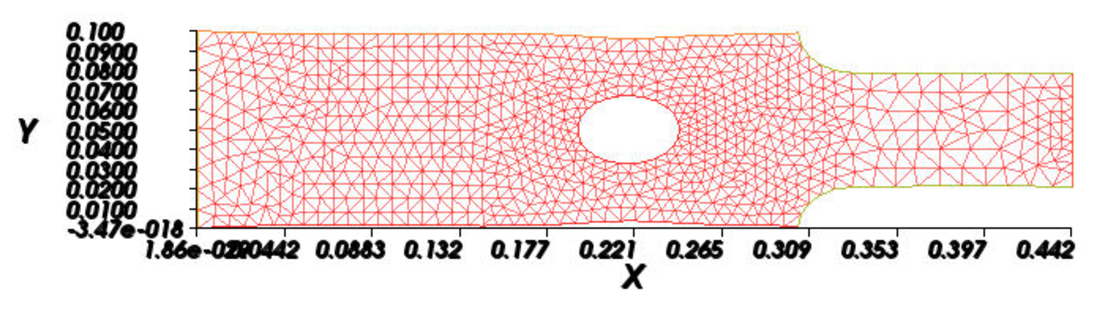
\includegraphics[width=1\textwidth]{paper/4-2-4.pdf}
\caption{Tấm kim loại dưới tác dụng của lực kéo F=1e4.}
\label{fig:exam24}
\end{figure}
\subsection{Mô phỏng thí nghiệm với lực nén}
Xét một tấm kim loại có một lỗ ở giữa chịu tác động của một lực nén $f=(-1e4,0)$ và trọng lực $g=(0,-9.81)$. Cho hằng số mô-đun đàn hồi Young $E=7e4$ và hệ số Poisson $v=0,3$ \cite{TIT-07}. Ta có hình \eqref{fig:exam31} - khởi tạo lưới ban đầu của tấm kim loại và hình \eqref{fig:exam32} - thể hiện lưới biến dạng của tấm kim loại sau khi chịu tác động bởi lực nén.\\
\begin{figure}[http]
\centering
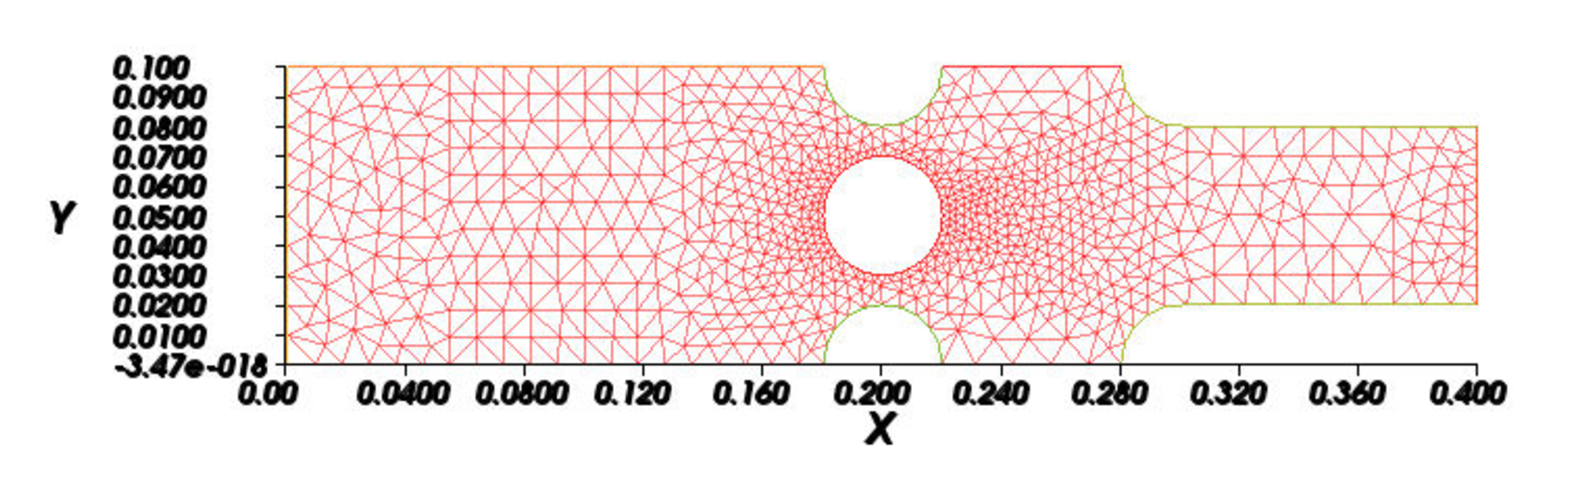
\includegraphics[width=1\textwidth]{paper/4-3-1.pdf}
\caption{Tấm kim loại ở trạng thái ban đầu.}
\label{fig:exam31}
\end{figure}
\begin{figure}[http]
\centering
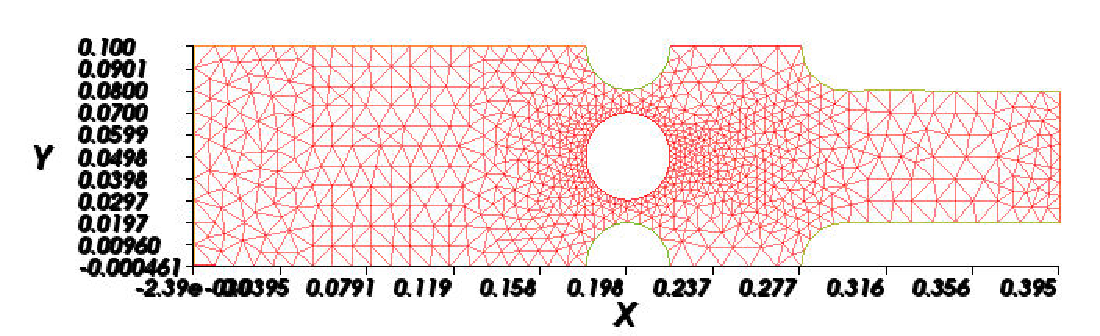
\includegraphics[width=1\textwidth]{paper/4-3-2.pdf}
\caption{Tấm kim loại dưới tác dụng của lực nén.}
\label{fig:exam32}
\end{figure}\\

Xét một tấm kim loại có kích thước là $2 \times 2$ với đáy cố định, chịu tác dụng của một lực nén $f = (0,-1e7)$ lên phía trên của tấm kim loại. Tấm kim loại có một lỗ được cho bởi phương trình $r = 0.5 + 0.2 sin(kt)$ trong tọa độ cực. Trong ví dụ này, ta xét $k=5$. Cho hằng số mô-đun đàn hồi Young và hệ số Poisson lần lượt bằng $E=1e9;\; v=0,3$. Dưới đây là lưới khởi tạo với 5796 tam giác của tấm kim loại \ref{fig:exam33}:\\

\begin{figure}[http]
\centering
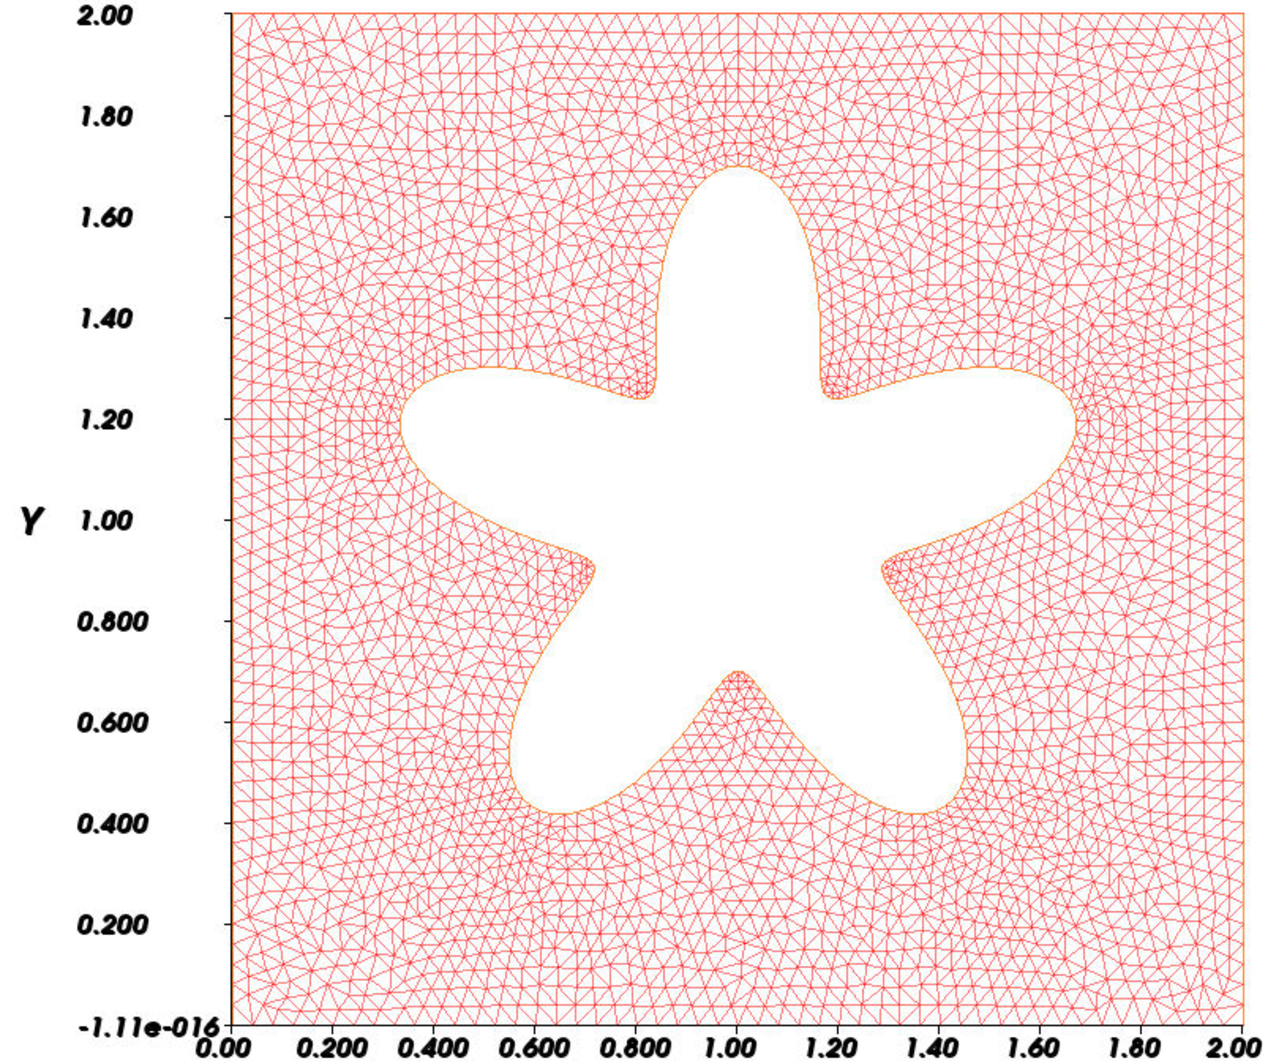
\includegraphics[width=0.6\textwidth]{paper/4-3-3.pdf}
\caption{Tấm kim loại $2 \times 2$ với lỗ $r = 0.5 + 0.2 sin(kt)$.}
\label{fig:exam33}
\end{figure}
Dưới tác dụng của lực nén, tấm sẽ bị nén theo chiều y và phình to ra theo hướng x. Hình sau biểu thị sự dịch chuyển biến dạng của tấm kim loại:\\
\begin{figure}[http]
\centering
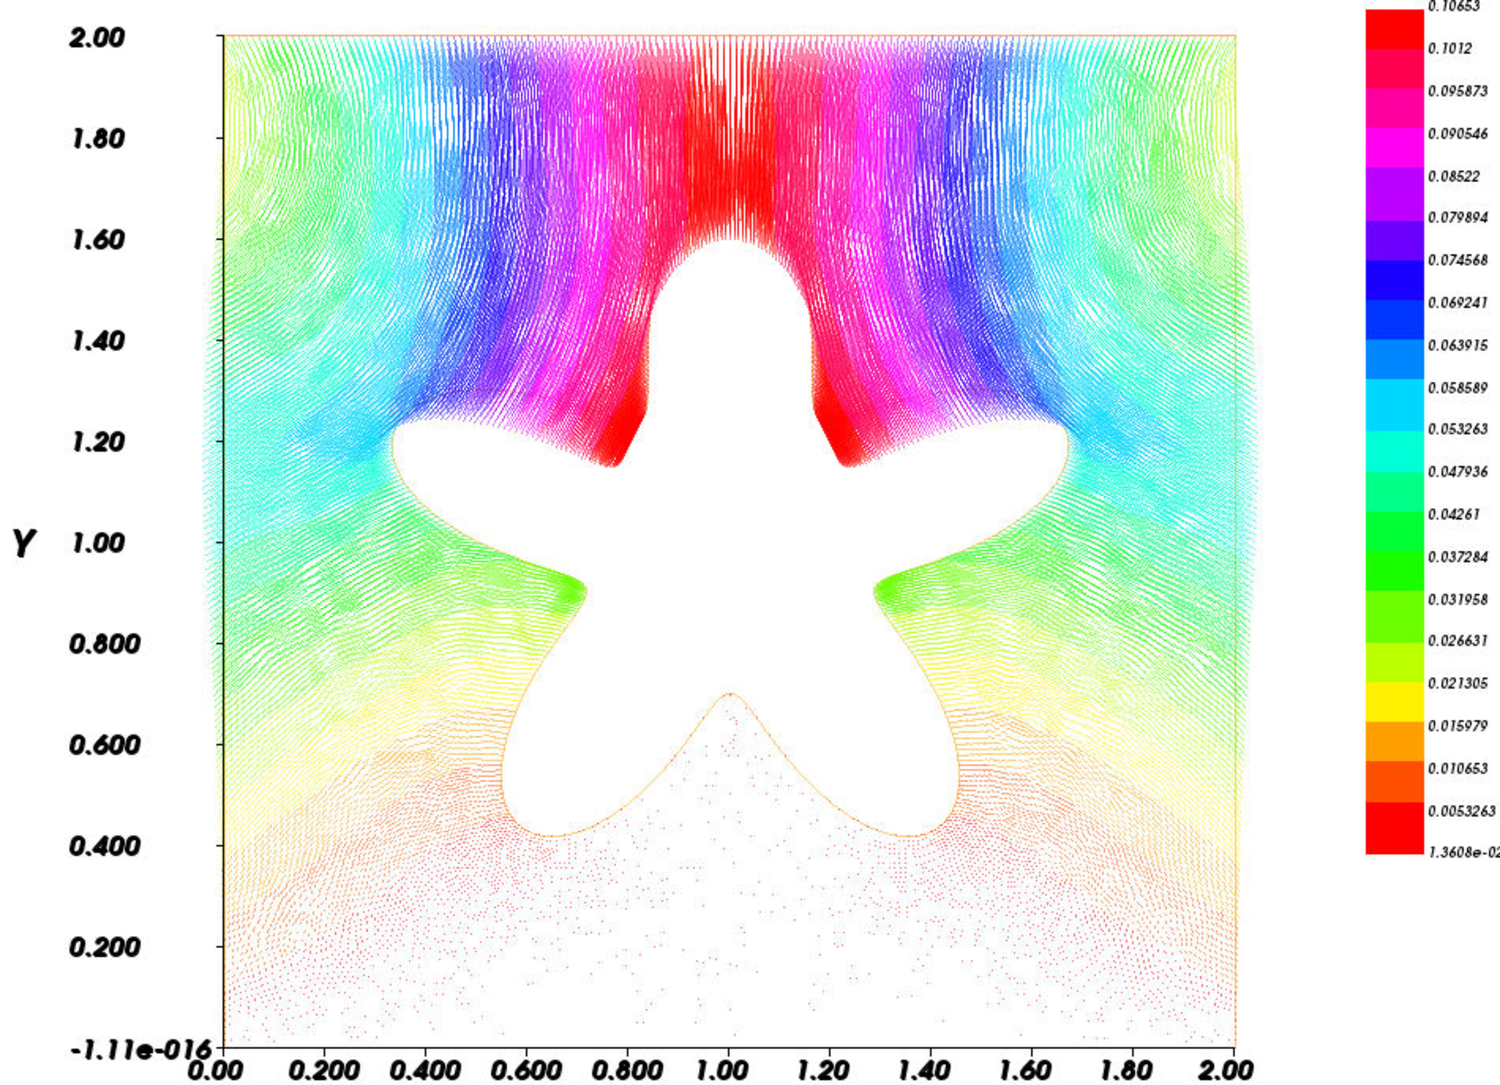
\includegraphics[width=0.6\textwidth]{paper/4-3-4.pdf}
\caption{Hướng dịch chuyển của tấm kim loại.}
\label{fig:exam34}
\end{figure}\\
\begin{figure}[http]
\centering
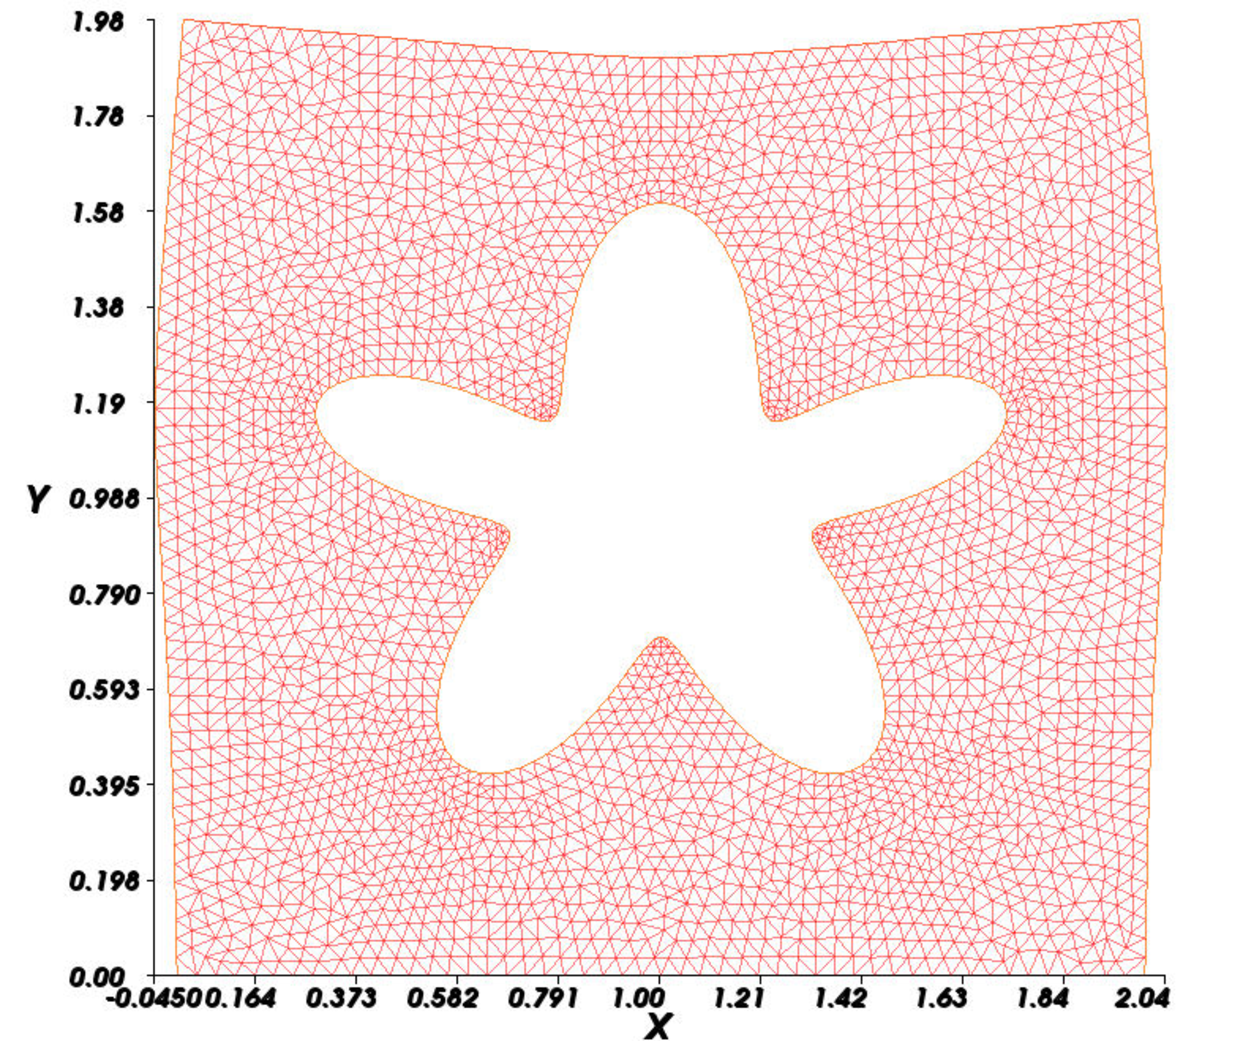
\includegraphics[width=0.6\textwidth]{paper/4-3-5.pdf}
\caption{Tấm kim loại sau khi bị biến dạng.}
\label{fig:exam35}
\end{figure}\\
\subsection{Mô phỏng thí nghiệm với áp suất}
Một tấm kim loại hình khuyên phải chịu một áp lực bên trong như hình \ref{fig:exam41} với $p=1e3;\;E=2e5;\;v=0.3;\;r_i=42;\;r_e=50;\;h=1 (h<<r_i)$ \cite{TIT-07}. Do $(h<<r_i)$ nên ta có thể coi đây là một bài toán 2 chiều. Ở ví dụ tiếp theo, ta xét một ống kim loại có cùng $p, E, v, r_i, r_e$ với chiều dài không nhỏ hơn quá nhiều so với bán kính của ống. Khi đó, bài toán trở thành bài toán 3 chiều.
\begin{figure}[http]
\centering
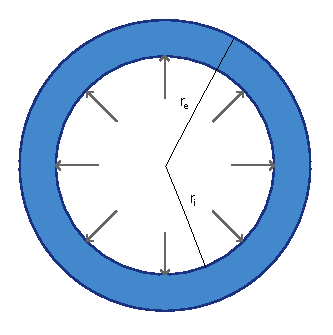
\includegraphics[width=0.4\textwidth]{paper/4-4.pdf}
\caption{Khuyên kim loại chịu tác động của áp suất ở bên trong.}
\label{fig:exam40}
\end{figure}\\
Hình \ref{fig:exam40} biểu diễn trạng thái ban đầu của khuyên kim loại và các lực tác động lên nó. Lưới khởi tạo và sự biến dạng của khuyên kim loại được biểu diễn như trong hình \ref{fig:exam41} \ref{fig:exam42}:
\begin{figure}[http]
\centering
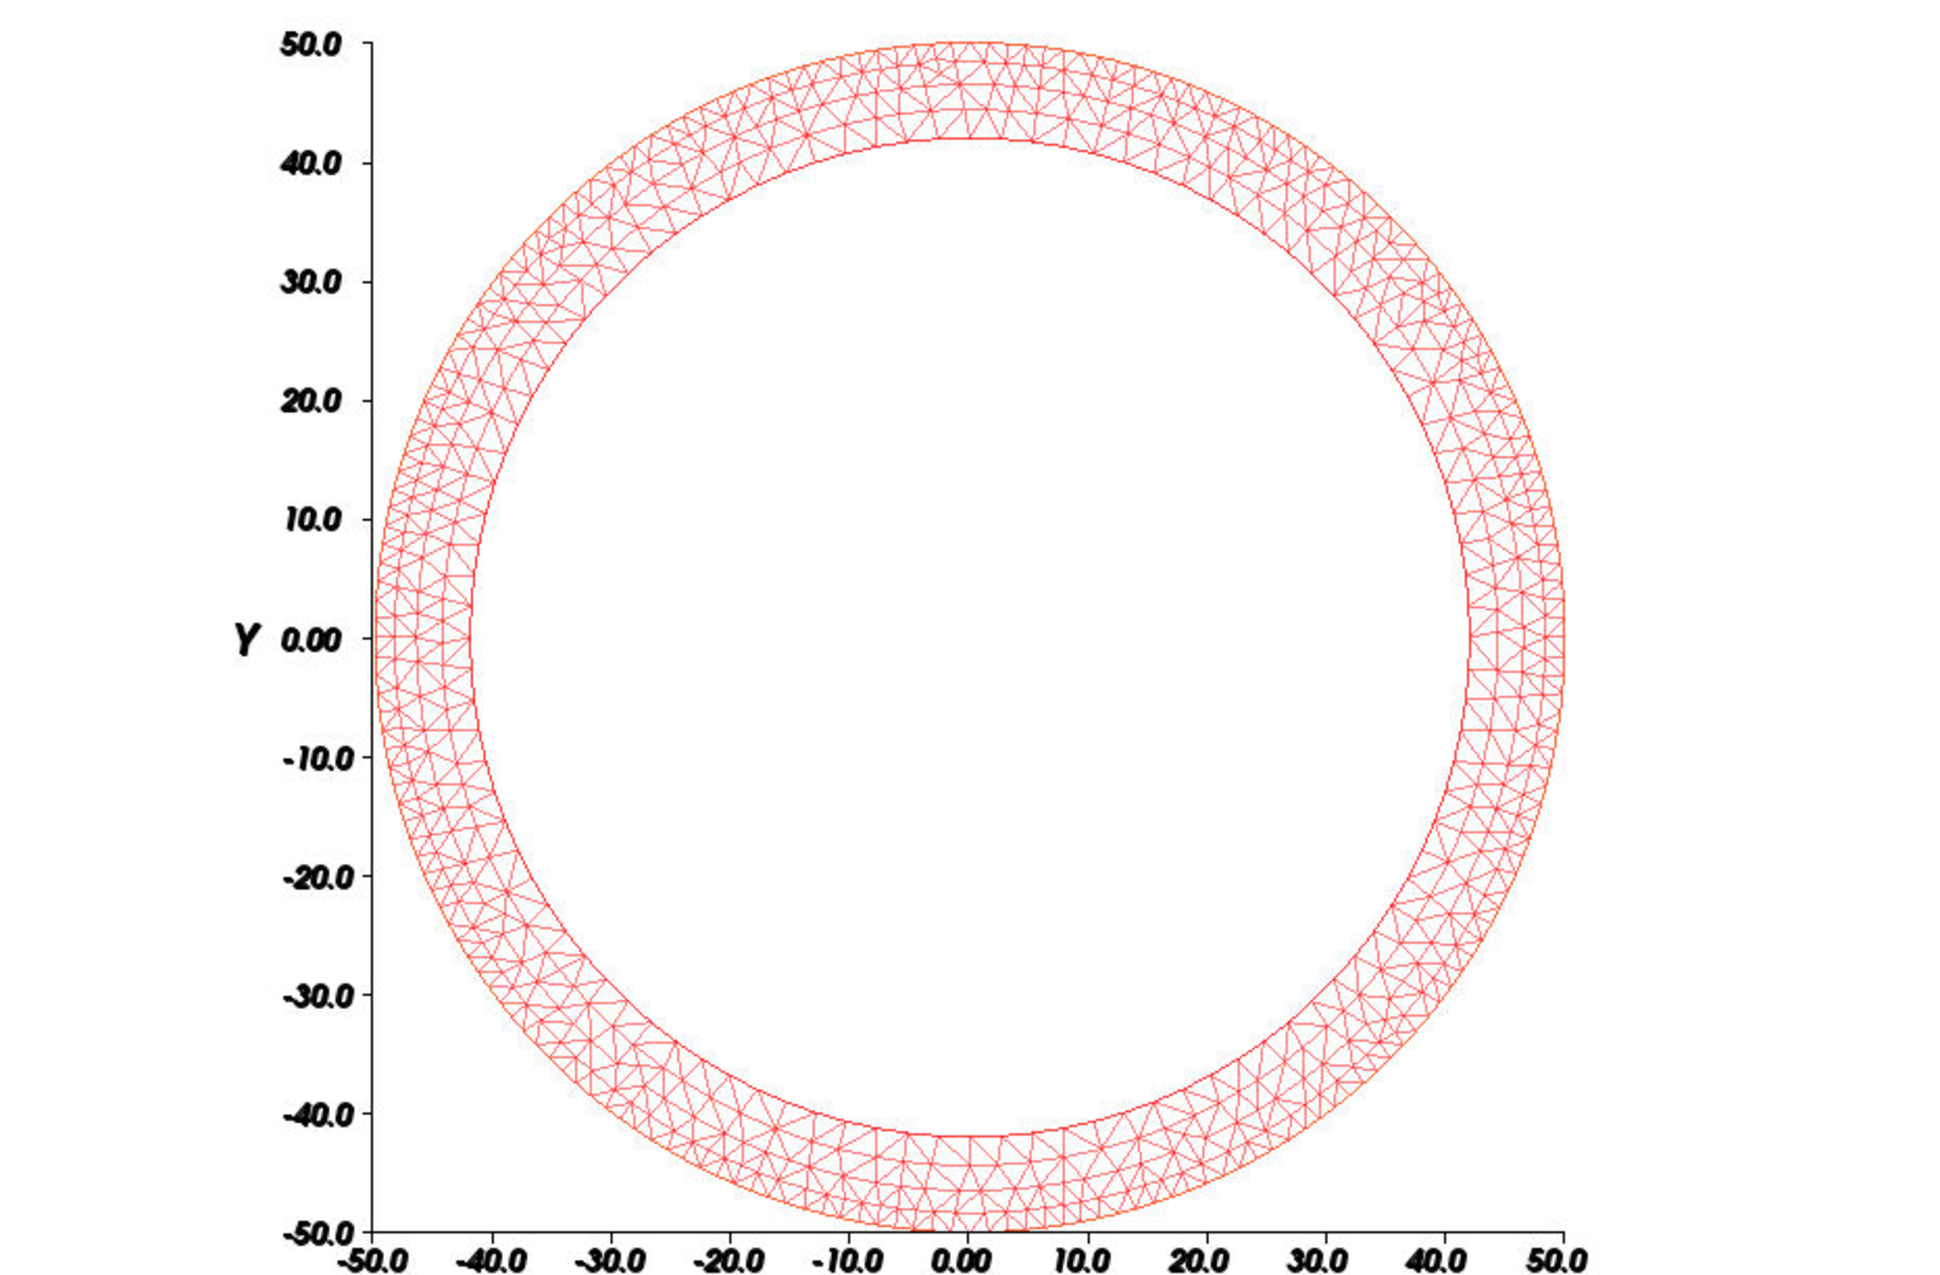
\includegraphics[width=0.6\textwidth]{paper/4-4-1.pdf}
\caption{Lưới khởi tạo của khuyên kim loại.}
\label{fig:exam41}
\end{figure}\\
\begin{figure}[http]
\centering
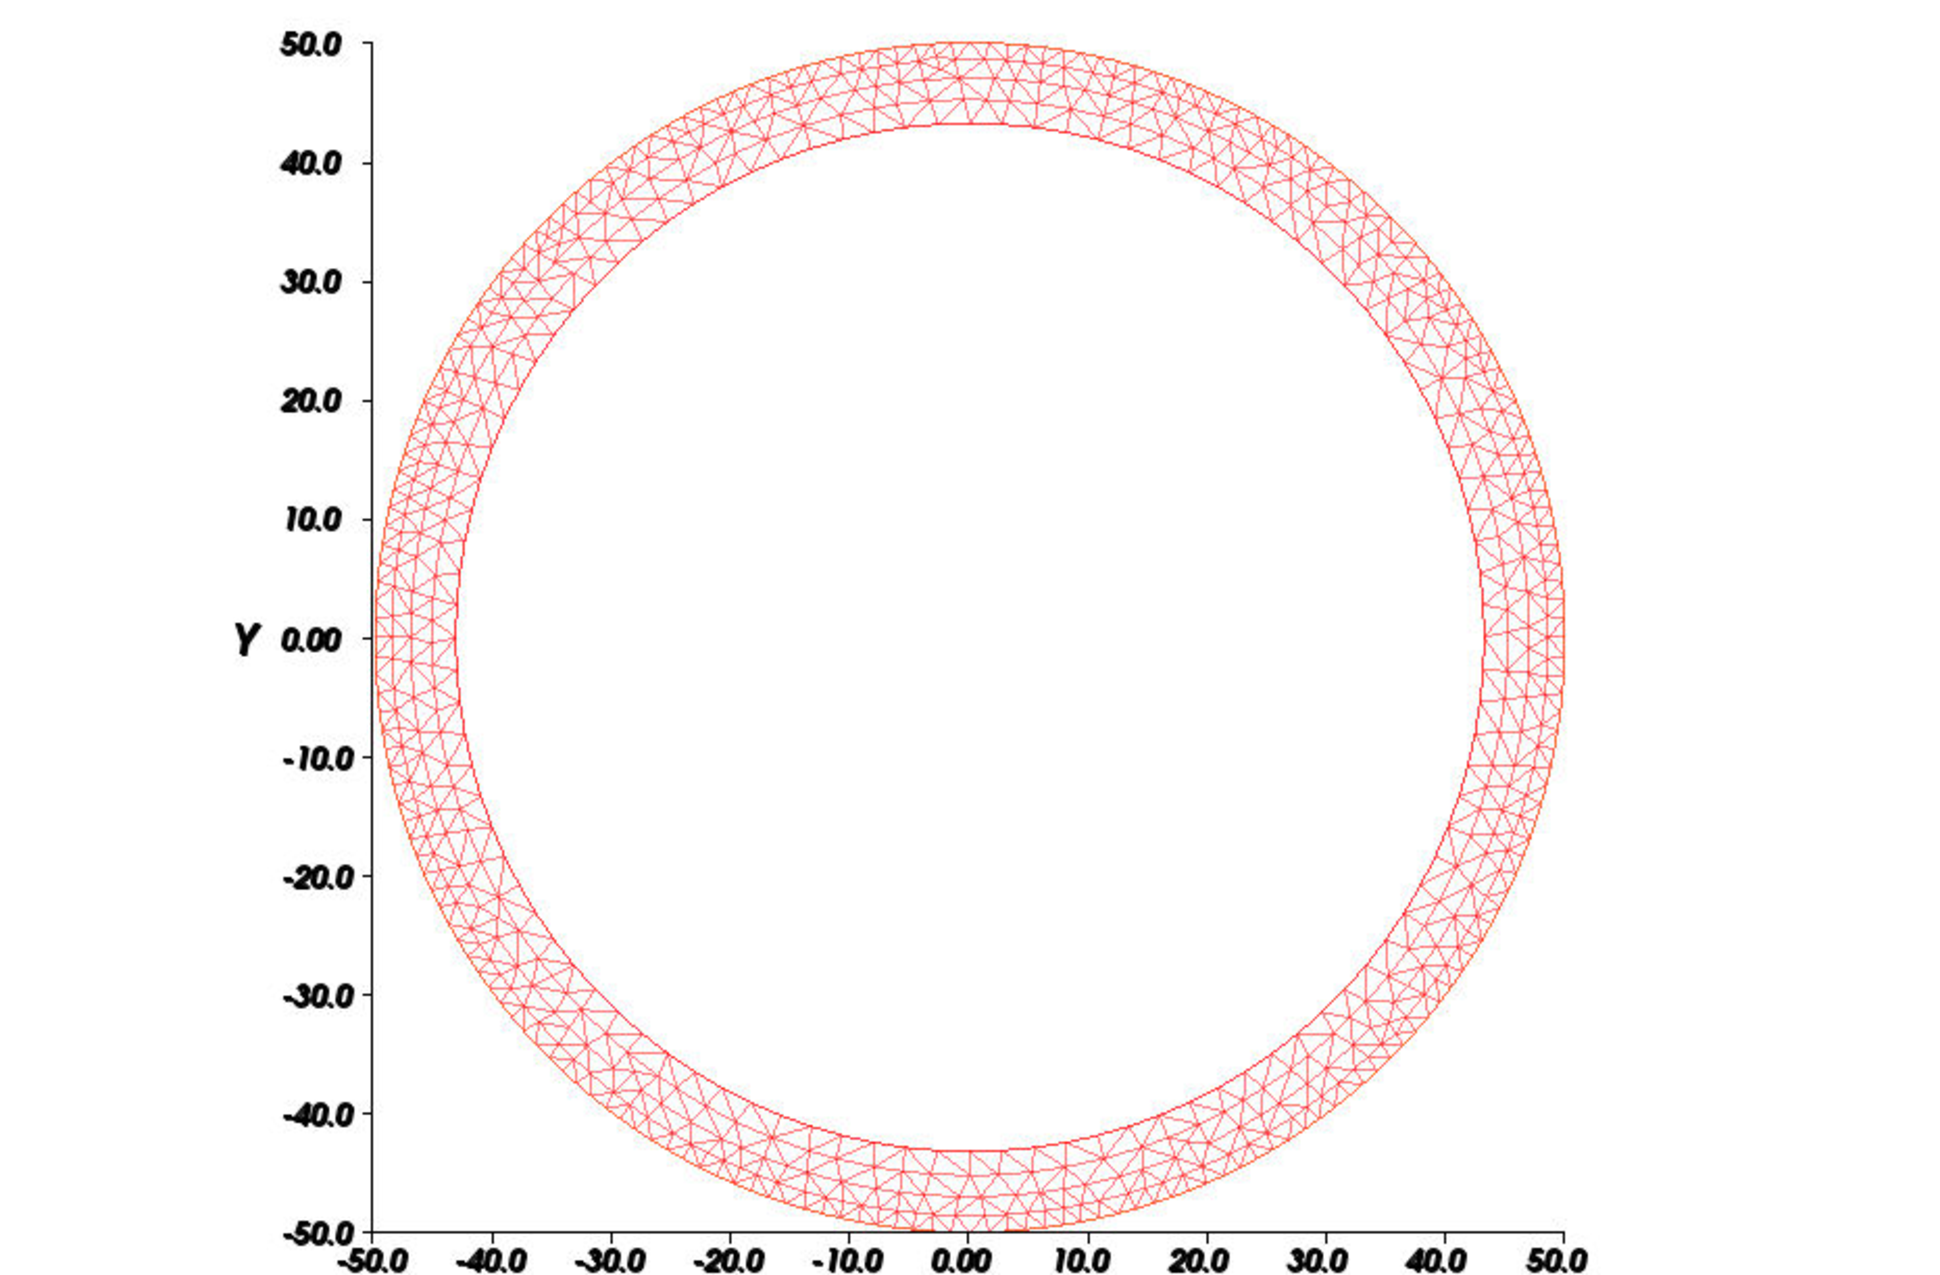
\includegraphics[width=0.6\textwidth]{paper/4-4-2.pdf}
\caption{Sự biến dạng của khuyên kim loại.}
\label{fig:exam42}
\end{figure}\\
Như đã nói ở trên, ta xét một ống kim loại. Có áp suất bên trong ống $p=1e3;\;E=2e5;\;v=0.3;\;r_i=40;\;r_e=50$ và ống có chiều dài $h=40$.\\
\begin{figure}[http]
\centering
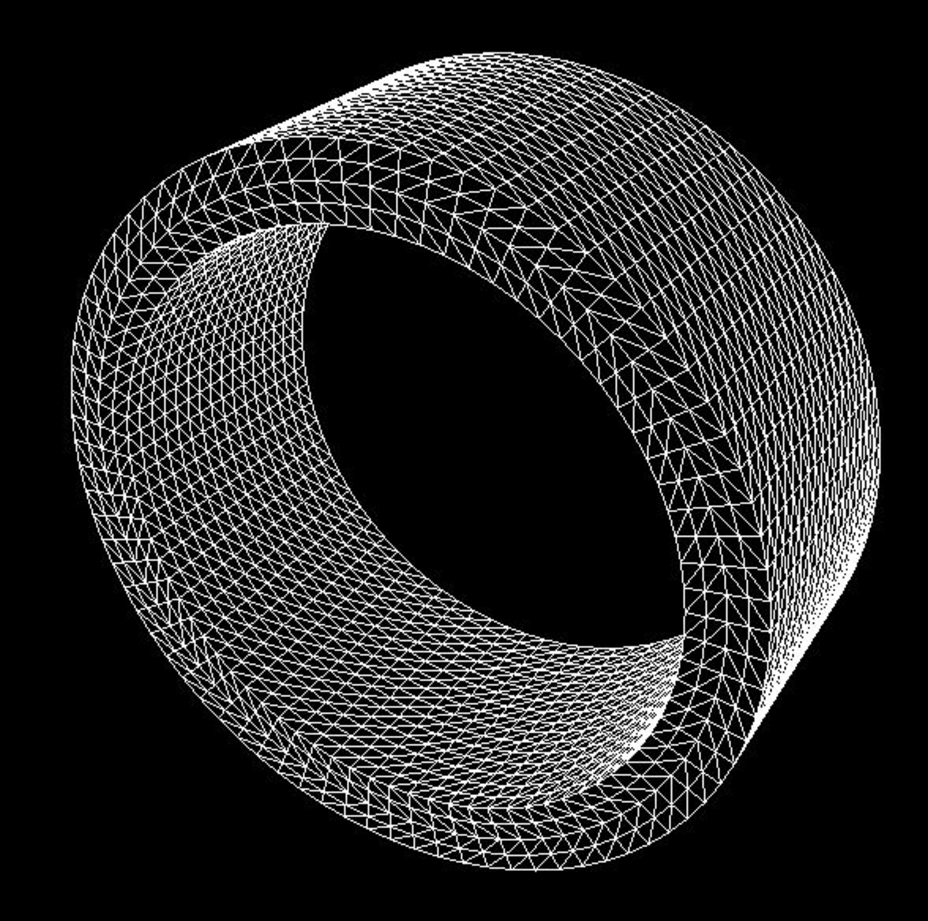
\includegraphics[width=0.6\textwidth]{paper/4-5.pdf}
\caption{Lưới khởi tạo của ống kim loại.}
\label{fig:exam50}
\end{figure}\\
Và các hình \ref{fig:exam51}, \ref{fig:exam52} cho thấy sự biến dạng của ống kim loại:
\begin{figure}[http]
\centering
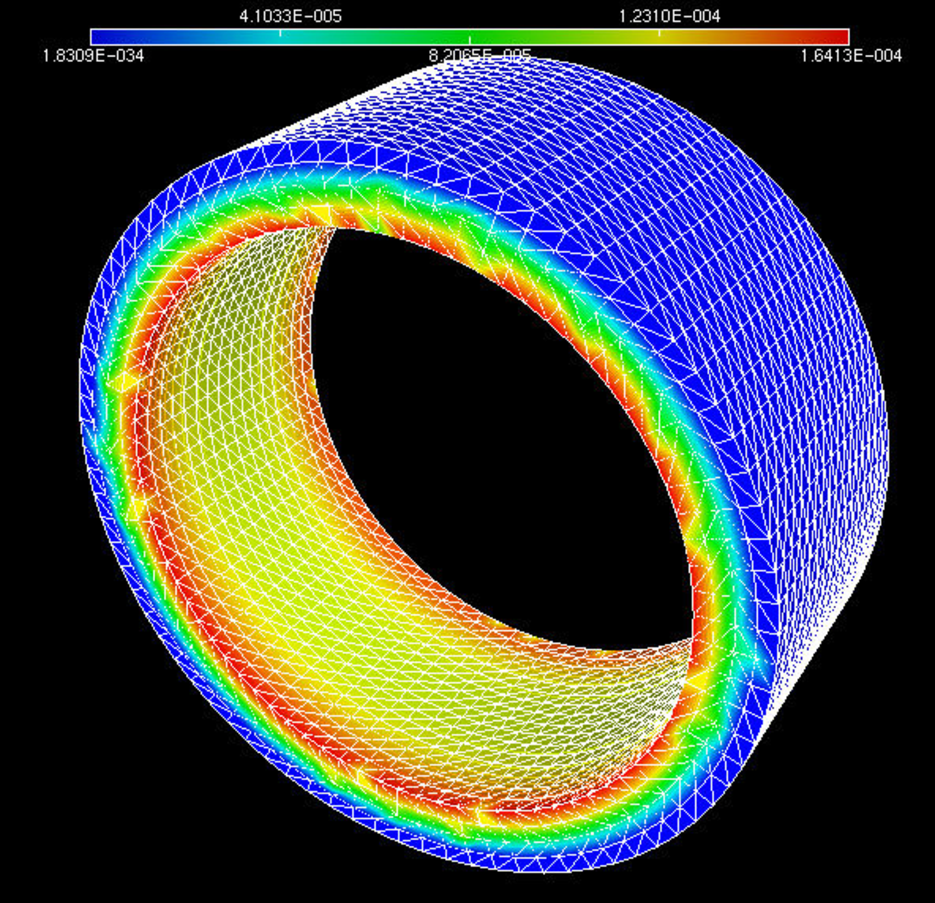
\includegraphics[width=0.6\textwidth]{paper/4-5-1.pdf}
\caption{Ống kim loại trước khi bị biến dạng.}
\label{fig:exam51}
\end{figure}\\
\begin{figure}[http]
\centering
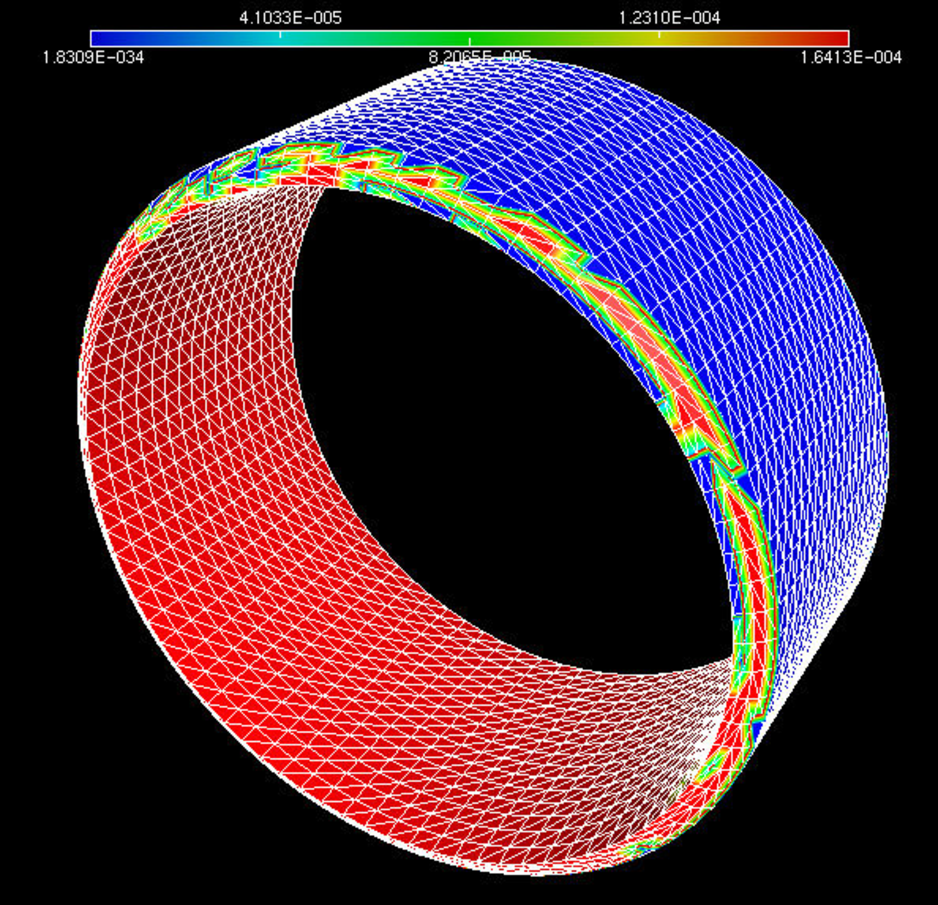
\includegraphics[width=0.6\textwidth]{paper/4-5-2.pdf}
\caption{Ống kim loại sau khi bị biến dạng.}
\label{fig:exam52}
\end{figure}\\

\section{Kết luận}
Trong chương này, ta đã trình bày chi tiết các bước xây dựng lược đồ giải số cho hệ phương trình biến dạng đàn hồi. Cụ thể, nội dung chương \ref{Chapter1} đã giải quyết những vấn đề sau:
\begin{itemize}
\item Phát biểu bài toán biến dạng đàn hồi.
\item Áp dụng phương pháp phần tử hữu hạn rời rạc hóa không gian, từ đó xây dựng bài toán rời rạc và hệ phương trình đại số tương ứng.
\item Trình bày các ví dụ giải số minh họa.
\end{itemize}

%----------------------------------------------------------------------------------------
% Chapter 2
\chapter{Ứng dụng trong công nghiệp vật liệu}\label{Chapter2}
\renewcommand{\baselinestretch}{1.25}
\minitoc
\renewcommand{\baselinestretch}{1.5}
%----------------------------------------------------------------------------------------
\section{Ứng dụng trong bài toán tối ưu dạng}
Trong sản xuất vật liệu công nghiệp, việc chọn được thành phần và thiết kế cấu trúc là một phẩn rất quan trọng để sản xuất các sản phẩm bền vững và mang tính cạnh tranh. Để đáp ứng các yêu cầu về độ bền của vật liệu, tối ưu hóa cấu trúc và cấu tạo của vật liệu được sử dụng quá trình thiết kế. Trong việc thiết kế vật liệu dựa trên tối ưu hóa hình dạng, thách thức chính ở đây là tuân theo hình dạng được đề xuất mà không tạo ra các biến thể phần thì quá mỏng dẹt hay phần thì quá dày quá dày gây nên mất hình dạng cấu trúc của vật. Do đó, tối ưu hình dạng vật liệu góp phần không nhỏ trong việc sản xuất vật liệu. Trong chương này của luận văn, phần đầu sẽ sẽ giới thiệu về bài toán tối ưu hình dạng của vật có cấu trúc đàn hồi và sau đó là một vài ví dụ mô phỏng số trong việc thiết kế cấu tạo của một số vật liệu.
\subsection{Bài toán tối ưu dạng}
Bài toán tối ưu dạng là bài toán tìm hình dạng tối ưu $\Omega^*$ của vật thể trong tập các hình dạng chấp nhận được $\Omega_x\subset\mathbb{R}^n$ theo một tiêu chí xác định nào đó và được mô tả thông qua việc cực tiểu hàm mục tiêu $J:\Omega_x\rightarrow\mathbb{R}$. Xét bài toán tối ưu dạng:
\begin{equation}\label{bt:toiuidang}
\inf_{\Omega\in\Omega_x}J(\Omega)
\end{equation}
Trong từng bài toán tối ưu dạng cụ thể, ta có được hàm mục tiêu $J(\Omega)$ khác nhau tương ứng trong các trường hợp đó. Chẳng hạn, khi ta cần tối ưu dạng của một đường ống (hình \ref{fig:exampipe}), ta quan tâm đến tổng công của dòng chảy được sinh ra bên trong ống:
$$J(\Omega) = 2\mu\int_\Omega D(u_\Omega):D(u_\Omega)dx.$$
\begin{figure}[http]
\centering
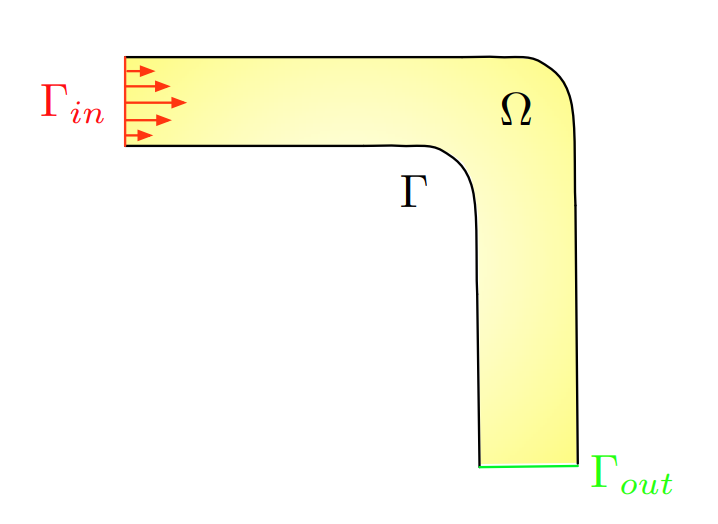
\includegraphics[width=0.6\textwidth]{exampipe.png}
\caption{Hình dạng ban đầu của đường ống.}
\label{fig:exampipe}
\end{figure}\\
Trong bài toán này, ta có thêm ràng buộc về thể tích cần đạt được cho đường ống để khống chế hình dạng tối ưu của đường ống.\\
Hàm bình phương sai số cũng là một hàm mục tiêu được xét nhiều trong các bài toán tối ưu hình dạng của các vật liệu. Ví dụ như ta xét một dòng chảy trên miền D, trong dòng chảy đó có một vật cản $\omega$ có hình dạng không xác định. Gọi $u_{meas}$ là vận tốc của dòng chảy $u_\Omega$ ở vị trí $\mathcal{O}$ với mục đích  tái cấu trúc hình dạng của vật cản $\omega$(hình \ref{fig:examdcvc}). Khi đó miền tối ưu là $\Omega = D\backslash\omega$ và chỉ phần $\partial\omega$ của $\partial\Omega$ là được tối ưu. Mục tiêu là ta cần tối thiểu hàm bình phương sai số:
$$J(\Omega)=\int_\mathcal{O}|u_\Omega - u_{meas}|^2dx.$$
\begin{figure}[http]
\centering
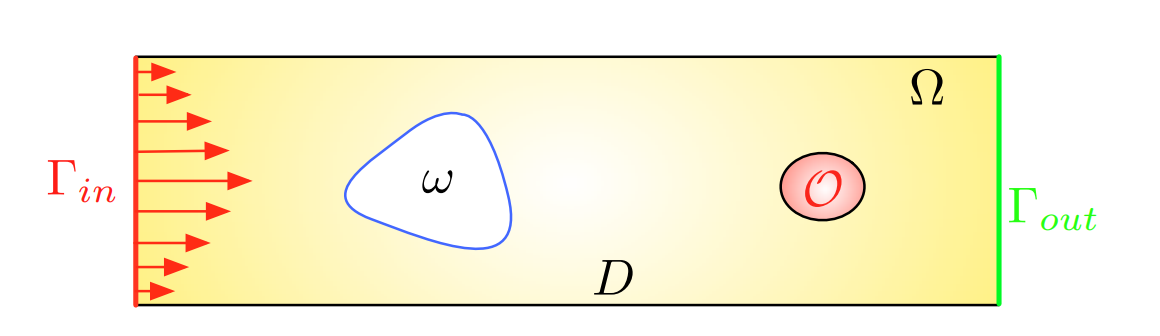
\includegraphics[width=0.8\textwidth]{examdcvc.png}
\caption{Dòng chảy trên miền $D$ có vật cản $\omega$ ở giữa.}
\label{fig:examdcvc}
\end{figure}\\
Trong ngành công nghiệp hàng không, hàm mục tiêu ở đây là ta cần tối ưu lực kéo $\mathcal{T}$ của cánh $\Omega$ \cite{Pir84, MP10}:
$$J(\Omega)=\mathcal{T}(\Omega)=\int_\Om \left[\mu \left(\nabla u + \nabla u^T\right) - \frac{2\mu}{3} \Div u \right]\nv \,dx  - \int_\Om p\nv \,dx.$$
Trong luận văn này, ta sẽ tìm hiểu rõ hơn về hàm mục tiêu dạng mô tả tính đàn hồi được áp dụng trong các bài toán tối ưu hóa hình dạng, cấu trúc vật liệu:
$$J(\Omega)=\int_\Omega f\cdot u\,dx + \int_{\Gm_N} g \cdot u \,ds = \int_{\Om} Ae(u):e(u)\,dx.$$

\subsection*{Các điều kiện ràng buộc}
Trong các ví dụ ở trên, ta có đề cập đến ràng buộc về thể tích tối ưu cần đạt được giúp ta khống chế được hình dạng cũng như cấu trúc của vật liệu. Ngoài ràng buộc về thể tích ra, trong bài toán tối ưu hình dạng của vật liệu, ta còn có điều kiện về chu vi dạng hay tổng độ cong biên.
\begin{itemize}
\item Thể tích dạng: $\text{Vol}(\Omega)=\int_\Omega dx$
\item Chu vi dạng: $\text{Per}(\Omega)=\int_{\partial\Omega} ds$
\item Tổng độ cong biên: $\mathcal{K}(\Omega)=\int_\Omega\kappa^2ds$
\end{itemize}
Đó là các hàm dạng phổ biến được sử dụng, đóng vai trò quan trọng việc hiệu chỉnh các thành phần của vật liệu cũng như tái cấu trúc hình dạng vật liệu.
\subsection*{Phương pháp Lagrange giải bài toán tối ưu có ràng buộc}
Để xử lý các điều kiện ràng buộc như đã đề cập ở trên, ta đưa nhân tử Lagrange $l$ vào hàm mục tiêu phương pháp đó còn gọi là phương pháp Lagrange tăng cường (Augmented Lagrange method) dùng để giải các bài toán tối ưu có ràng buộc. 
\subsection*{Phương pháp biến phân Hadamard}
\subsection*{Đạo hàm dạng của hàm mục tiêu}
\subsection*{Thuật toán tối ưu dạng}
\subsubsection*{Phương pháp gradient giải bài toán tối ưu}
\subsubsection*{Tính toán hướng giảm}
\subsection{Các ví dụ mô phỏng số}

%-----------------------------------------------------------
\section{Kết luận}
%\include{Chapters/Chapter2} 
%% Chapter 2
\chapter*{\centering Kết luận chung} % Main chapter title 
\addstarredchapter{Kết luận chung}

Luận văn này trình bày một lược đồ giải số cho bài toán tối ưu dạng trong cơ học chất lỏng, dựa trên phương pháp biến phân Hadamard và phương pháp phần tử hữu hạn. Cụ thể, luận văn đã giải quyết những vấn đề sau:
\begin{itemize}
\item Xây dựng lược đồ mô phỏng số cho hệ phương trình Navier-Stokes, dựa trên phương pháp đặc trưng và phương pháp phần tử hữu hạn.
\item Đề xuất thuật toán giải số cho bài toán tối ưu dạng trong dòng chảy Stokes.
\item Mô phỏng các thí nghiệm giải số minh họa.
\end{itemize}

Lược đồ giải số được đề xuất cho bài toán tối ưu dạng trong cơ học chất lỏng có những ưu điểm sau đây:
\begin{itemize}
\item Cho phép thực hiện các biến dạng phức tạp trong quá trình tối ưu.
\item Dễ dàng mở rộng để giải quyết cho các hình dạng khác nhau, các hàm mục tiêu cũng như các mô hình cơ học khác, chẳng hạn như mô hình đàn hồi tuyến tính, dòng đối lưu tự nhiên, \ldots.
\item Chi phí của thuật toán là vừa phải.
\end{itemize}

Tính hiệu quả và độ tin cậy có lược đồ đã được thể hiện qua năm thí nghiệm giải số. Tuy nhiên, thuật toán này cũng có những nhược điểm như sau:
\begin{itemize}
\item Dạng tối ưu thu được phụ thuộc nhiều vào hình dạng ban đầu. 
\item Thuật toán chỉ làm thay đổi hình dạng chứ không làm thay đổi topology của miền.
\end{itemize} 

%----------------------------------------------------------------------------------------
\chapter*{\centering Các hướng nghiên cứu tiếp theo}
\addstarredchapter{Các hướng nghiên cứu tiếp theo}
Tác giả đề xuất các hướng nghiên cứu liên quan có thể tiếp tục phát triển từ nội dung của luận văn này:
\begin{itemize}
\item Mô phỏng các thí nghiệm giải số cho hệ phương trình Navier-Stokes cũng như cho bài toán tối ưu dạng trong không gian ba chiều.
\item Xây dựng thuật toán tìm bước giảm tối ưu.
\item Kết hợp sử dụng phương pháp tập mức ({\em level set method}) cho bài toán tối ưu dạng để thay đổi topology của miền, như được trình bày trong nghiên cứu \cite{AJT04}.
\item Mở rộng lược đồ giải số cho dòng chảy Navier-Stokes như trong \cite{DMZ08b}, cũng như xem xét các hàm mục tiêu khác, chẳng hạn hàm cực tiểu bình phương sai số hoặc cực đại tính thấm, được đề cập trong nghiên cứu \cite{ZL08}.
\item Áp dụng lược đồ hiện tại để giải quyết các bài toán ứng dụng tối ưu dạng trong nhiều mô hình vật lý khác nhau, chẳng hạn như các cấu trúc đàn hồi \cite{AJT04, Dap13}, cấu trúc truyền nhiệt \cite{YWM13}, dòng đối lưu tự nhiên \cite{AAA+14}.
\end{itemize}

Dựa trên cách tiếp cận của thuật toán đề xuất, trong quá trình thực hiện luận văn này, tác giả đã nghiên cứu xây dựng lược đồ giải số cho bài toán tối ưu dạng trong cấu trúc đàn hồi tuyến tính và đã đạt được những kết quả nhất định. Tuy nhiên, do hạn chế về thời gian thực hiện nên nghiên cứu này vẫn đang trong quá trình tiếp tục hoàn thiện.

%----------------------------------------------------------------------------------------
\chapter*{\centering Danh mục các công trình liên quan đến luận văn đã công bố}
\addstarredchapter{Danh mục các công trình liên quan đến luận văn đã công bố}
\begin{itemize}
\item[1.] L.V. Chien, N.H. Du, T.T.T. Mai, T.M. Tam. “Characteristic finite element method for natural convection problems”. May 2018. ({\em đã gửi đăng})
\item[2.] T.T.T. Mai, L.V. Chien, and P.H. Thanh. “Shape optimization for Stokes flows using sensitivity analysis and finite element method”. \textit{Applied Numerical Mathematics}. 126 (2018), pp. 160 –179. ISSN: 0168-9274.
\end{itemize}

%----------------------------------------------------------------------------------------


%\printbibliography
%\addstarredchapter{Tài liệu tham khảo}


%----------------------------------------------------------------------------------------
\end{document}  
